% Options for packages loaded elsewhere
\PassOptionsToPackage{unicode}{hyperref}
\PassOptionsToPackage{hyphens}{url}
\PassOptionsToPackage{dvipsnames,svgnames,x11names}{xcolor}
%
\documentclass[
  letterpaper,
]{krantz}

\usepackage{amsmath,amssymb}
\usepackage{iftex}
\ifPDFTeX
  \usepackage[T1]{fontenc}
  \usepackage[utf8]{inputenc}
  \usepackage{textcomp} % provide euro and other symbols
\else % if luatex or xetex
  \usepackage{unicode-math}
  \defaultfontfeatures{Scale=MatchLowercase}
  \defaultfontfeatures[\rmfamily]{Ligatures=TeX,Scale=1}
\fi
\usepackage{lmodern}
\ifPDFTeX\else  
    % xetex/luatex font selection
\fi
% Use upquote if available, for straight quotes in verbatim environments
\IfFileExists{upquote.sty}{\usepackage{upquote}}{}
\IfFileExists{microtype.sty}{% use microtype if available
  \usepackage[]{microtype}
  \UseMicrotypeSet[protrusion]{basicmath} % disable protrusion for tt fonts
}{}
\makeatletter
\@ifundefined{KOMAClassName}{% if non-KOMA class
  \IfFileExists{parskip.sty}{%
    \usepackage{parskip}
  }{% else
    \setlength{\parindent}{0pt}
    \setlength{\parskip}{6pt plus 2pt minus 1pt}}
}{% if KOMA class
  \KOMAoptions{parskip=half}}
\makeatother
\usepackage{xcolor}
\setlength{\emergencystretch}{3em} % prevent overfull lines
\setcounter{secnumdepth}{5}
% Make \paragraph and \subparagraph free-standing
\makeatletter
\ifx\paragraph\undefined\else
  \let\oldparagraph\paragraph
  \renewcommand{\paragraph}{
    \@ifstar
      \xxxParagraphStar
      \xxxParagraphNoStar
  }
  \newcommand{\xxxParagraphStar}[1]{\oldparagraph*{#1}\mbox{}}
  \newcommand{\xxxParagraphNoStar}[1]{\oldparagraph{#1}\mbox{}}
\fi
\ifx\subparagraph\undefined\else
  \let\oldsubparagraph\subparagraph
  \renewcommand{\subparagraph}{
    \@ifstar
      \xxxSubParagraphStar
      \xxxSubParagraphNoStar
  }
  \newcommand{\xxxSubParagraphStar}[1]{\oldsubparagraph*{#1}\mbox{}}
  \newcommand{\xxxSubParagraphNoStar}[1]{\oldsubparagraph{#1}\mbox{}}
\fi
\makeatother


\providecommand{\tightlist}{%
  \setlength{\itemsep}{0pt}\setlength{\parskip}{0pt}}\usepackage{longtable,booktabs,array}
\usepackage{calc} % for calculating minipage widths
% Correct order of tables after \paragraph or \subparagraph
\usepackage{etoolbox}
\makeatletter
\patchcmd\longtable{\par}{\if@noskipsec\mbox{}\fi\par}{}{}
\makeatother
% Allow footnotes in longtable head/foot
\IfFileExists{footnotehyper.sty}{\usepackage{footnotehyper}}{\usepackage{footnote}}
\makesavenoteenv{longtable}
\usepackage{graphicx}
\makeatletter
\newsavebox\pandoc@box
\newcommand*\pandocbounded[1]{% scales image to fit in text height/width
  \sbox\pandoc@box{#1}%
  \Gscale@div\@tempa{\textheight}{\dimexpr\ht\pandoc@box+\dp\pandoc@box\relax}%
  \Gscale@div\@tempb{\linewidth}{\wd\pandoc@box}%
  \ifdim\@tempb\p@<\@tempa\p@\let\@tempa\@tempb\fi% select the smaller of both
  \ifdim\@tempa\p@<\p@\scalebox{\@tempa}{\usebox\pandoc@box}%
  \else\usebox{\pandoc@box}%
  \fi%
}
% Set default figure placement to htbp
\def\fps@figure{htbp}
\makeatother
% definitions for citeproc citations
\NewDocumentCommand\citeproctext{}{}
\NewDocumentCommand\citeproc{mm}{%
  \begingroup\def\citeproctext{#2}\cite{#1}\endgroup}
\makeatletter
 % allow citations to break across lines
 \let\@cite@ofmt\@firstofone
 % avoid brackets around text for \cite:
 \def\@biblabel#1{}
 \def\@cite#1#2{{#1\if@tempswa , #2\fi}}
\makeatother
\newlength{\cslhangindent}
\setlength{\cslhangindent}{1.5em}
\newlength{\csllabelwidth}
\setlength{\csllabelwidth}{3em}
\newenvironment{CSLReferences}[2] % #1 hanging-indent, #2 entry-spacing
 {\begin{list}{}{%
  \setlength{\itemindent}{0pt}
  \setlength{\leftmargin}{0pt}
  \setlength{\parsep}{0pt}
  % turn on hanging indent if param 1 is 1
  \ifodd #1
   \setlength{\leftmargin}{\cslhangindent}
   \setlength{\itemindent}{-1\cslhangindent}
  \fi
  % set entry spacing
  \setlength{\itemsep}{#2\baselineskip}}}
 {\end{list}}
\usepackage{calc}
\newcommand{\CSLBlock}[1]{\hfill\break\parbox[t]{\linewidth}{\strut\ignorespaces#1\strut}}
\newcommand{\CSLLeftMargin}[1]{\parbox[t]{\csllabelwidth}{\strut#1\strut}}
\newcommand{\CSLRightInline}[1]{\parbox[t]{\linewidth - \csllabelwidth}{\strut#1\strut}}
\newcommand{\CSLIndent}[1]{\hspace{\cslhangindent}#1}

\usepackage{booktabs}
\usepackage{longtable}
\usepackage{array}
\usepackage{multirow}
\usepackage{wrapfig}
\usepackage{float}
\usepackage{colortbl}
\usepackage{pdflscape}
\usepackage{tabu}
\usepackage{threeparttable}
\usepackage{threeparttablex}
\usepackage[normalem]{ulem}
\usepackage{makecell}
\usepackage{xcolor}
\makeatletter
\@ifpackageloaded{tcolorbox}{}{\usepackage[skins,breakable]{tcolorbox}}
\@ifpackageloaded{fontawesome5}{}{\usepackage{fontawesome5}}
\definecolor{quarto-callout-color}{HTML}{909090}
\definecolor{quarto-callout-note-color}{HTML}{0758E5}
\definecolor{quarto-callout-important-color}{HTML}{CC1914}
\definecolor{quarto-callout-warning-color}{HTML}{EB9113}
\definecolor{quarto-callout-tip-color}{HTML}{00A047}
\definecolor{quarto-callout-caution-color}{HTML}{FC5300}
\definecolor{quarto-callout-color-frame}{HTML}{acacac}
\definecolor{quarto-callout-note-color-frame}{HTML}{4582ec}
\definecolor{quarto-callout-important-color-frame}{HTML}{d9534f}
\definecolor{quarto-callout-warning-color-frame}{HTML}{f0ad4e}
\definecolor{quarto-callout-tip-color-frame}{HTML}{02b875}
\definecolor{quarto-callout-caution-color-frame}{HTML}{fd7e14}
\makeatother
\makeatletter
\@ifpackageloaded{bookmark}{}{\usepackage{bookmark}}
\makeatother
\makeatletter
\@ifpackageloaded{caption}{}{\usepackage{caption}}
\AtBeginDocument{%
\ifdefined\contentsname
  \renewcommand*\contentsname{Indice}
\else
  \newcommand\contentsname{Indice}
\fi
\ifdefined\listfigurename
  \renewcommand*\listfigurename{Elenco delle Figure}
\else
  \newcommand\listfigurename{Elenco delle Figure}
\fi
\ifdefined\listtablename
  \renewcommand*\listtablename{Elenco delle Tabelle}
\else
  \newcommand\listtablename{Elenco delle Tabelle}
\fi
\ifdefined\figurename
  \renewcommand*\figurename{Figura}
\else
  \newcommand\figurename{Figura}
\fi
\ifdefined\tablename
  \renewcommand*\tablename{Tabella}
\else
  \newcommand\tablename{Tabella}
\fi
}
\@ifpackageloaded{float}{}{\usepackage{float}}
\floatstyle{ruled}
\@ifundefined{c@chapter}{\newfloat{codelisting}{h}{lop}}{\newfloat{codelisting}{h}{lop}[chapter]}
\floatname{codelisting}{Lista}
\newcommand*\listoflistings{\listof{codelisting}{Elenco degli Elenchi}}
\makeatother
\makeatletter
\makeatother
\makeatletter
\@ifpackageloaded{caption}{}{\usepackage{caption}}
\@ifpackageloaded{subcaption}{}{\usepackage{subcaption}}
\makeatother

\ifLuaTeX
\usepackage[bidi=basic]{babel}
\else
\usepackage[bidi=default]{babel}
\fi
\babelprovide[main,import]{italian}
% get rid of language-specific shorthands (see #6817):
\let\LanguageShortHands\languageshorthands
\def\languageshorthands#1{}
\usepackage{bookmark}

\IfFileExists{xurl.sty}{\usepackage{xurl}}{} % add URL line breaks if available
\urlstyle{same} % disable monospaced font for URLs
\hypersetup{
  pdftitle={Psicometria},
  pdfauthor={Corrado Caudek},
  pdflang={it},
  colorlinks=true,
  linkcolor={blue},
  filecolor={Maroon},
  citecolor={Blue},
  urlcolor={Blue},
  pdfcreator={LaTeX via pandoc}}


\title{Psicometria}
\usepackage{etoolbox}
\makeatletter
\providecommand{\subtitle}[1]{% add subtitle to \maketitle
  \apptocmd{\@title}{\par {\large #1 \par}}{}{}
}
\makeatother
\subtitle{Anno Accademico 2024/2025}
\author{Corrado Caudek}
\date{2025-02-21}

\begin{document}
\maketitle

\renewcommand*\contentsname{Indice}
{
\hypersetup{linkcolor=}
\setcounter{tocdepth}{2}
\tableofcontents
}

\bookmarksetup{startatroot}

\chapter*{Benvenuti}\label{benvenuti}
\addcontentsline{toc}{chapter}{Benvenuti}

\markboth{Benvenuti}{Benvenuti}

Benvenuti nel sito web dell'insegnamento di
\href{https://www.unifi.it/index.php?module=ofform2&mode=1&cmd=3&AA=2023&afId=689762}{Psicometria},
parte del
\href{https://www.psicologia.unifi.it/vp-130-scienze-e-tecniche-psicologiche-l-24.html}{Corso
di Laurea in Scienze e Tecniche Psicologiche}
dell'\href{https://www.unifi.it/}{Università degli Studi di Firenze}.

\section*{Descrizione}\label{descrizione}
\addcontentsline{toc}{section}{Descrizione}

\markright{Descrizione}

Il corso offre una formazione teorico-pratica nell'analisi dei dati
psicologici, con particolare attenzione alle applicazioni in R. Vengono
affrontati temi come analisi descrittiva, esplorazione dei dati, flusso
di lavoro, organizzazione di progetti e modelli statistici di base, sia
bayesiani che frequentisti. Grande enfasi è posta sulle buone pratiche
di Open Science, promuovendo trasparenza e riproducibilità nelle
analisi.

\begin{itemize}
\tightlist
\item
  \textbf{Anno Accademico}: 2024-2025
\item
  \textbf{Codice Insegnamento}: B000286
\item
  \textbf{Orario e Luogo}: Lunedì e Martedì (8:30-10:30), Giovedì
  (11:30-13:30), Plesso didattico La Torretta.
\end{itemize}

\begin{tcolorbox}[enhanced jigsaw, toprule=.15mm, breakable, bottomrule=.15mm, colback=white, colbacktitle=quarto-callout-note-color!10!white, left=2mm, toptitle=1mm, colframe=quarto-callout-note-color-frame, coltitle=black, opacitybacktitle=0.6, bottomtitle=1mm, titlerule=0mm, leftrule=.75mm, opacityback=0, rightrule=.15mm, title=\textcolor{quarto-callout-note-color}{\faInfo}\hspace{0.5em}{Nota}, arc=.35mm]

Questo sito web ospita la dispensa ufficiale
dell'insegnamento~\textbf{B000286 - Psicometria}, che include tutte le
note e i materiali relativi alle lezioni.

\end{tcolorbox}

\section*{Struttura dell'Insegnamento}\label{struttura-dellinsegnamento}
\addcontentsline{toc}{section}{Struttura dell'Insegnamento}

\markright{Struttura dell'Insegnamento}

Il corso è strutturato per fornire una solida base teorica e pratica
nell'analisi dei dati psicologici, combinando approcci metodologici,
applicazioni pratiche ed esercitazioni mirate.

\begin{itemize}
\tightlist
\item
  \textbf{Introduzione a R}: Approccio pratico all'utilizzo di R per
  l'analisi dei dati, con enfasi sulla scrittura di script replicabili e
  sulla creazione di workflow efficienti.\\
\item
  \textbf{Gestione di Progetti di Analisi}: Strategie per organizzare,
  documentare e comunicare progetti di data analysis, seguendo le buone
  pratiche della Open Science e della ricerca trasparente.\\
\item
  \textbf{Statistica Descrittiva}: Esplorazione dei dati attraverso
  misure descrittive, distribuzioni statistiche e visualizzazioni
  grafiche.\\
\item
  \textbf{Fondamenti di Probabilità}: Introduzione ai concetti di
  probabilità, distribuzioni e incertezza, come base essenziale per
  l'inferenza statistica.\\
\item
  \textbf{Inferenza Frequentista e Bayesiana}: Panoramica sui due
  principali approcci all'inferenza statistica, con esempi pratici e
  confronto tra i metodi.\\
\item
  \textbf{Visualizzazione e Comunicazione}: Tecniche avanzate per
  rappresentare risultati statistici in modo chiaro, efficace e
  persuasivo, includendo la creazione di report e grafici professionali.
\end{itemize}

Il corso integra questi argomenti in un percorso didattico coerente, che
combina lezioni teoriche, esercitazioni pratiche e momenti di
riflessione critica. Gli studenti saranno così preparati ad applicare
l'analisi dei dati sia in contesti accademici che pratici.

\section*{Syllabus}\label{syllabus}
\addcontentsline{toc}{section}{Syllabus}

\markright{Syllabus}

\href{syllabus/syllabus.pdf}{Consulta il syllabus completo} per
ulteriori dettagli.

\bookmarksetup{startatroot}

\chapter*{Prefazione}\label{prefazione}
\addcontentsline{toc}{chapter}{Prefazione}

\markboth{Prefazione}{Prefazione}

Come possiamo migliorare l'analisi dei dati psicologici per renderla più
affidabile e robusta? È possibile affrontare questa sfida semplicemente
applicando una serie di algoritmi o procedure standard? L'analisi dei
dati in psicologia può davvero essere ridotta a un insieme di
``ricette'' preconfezionate
(\citeproc{ref-McElreath_rethinking}{McElreath, 2020})?

Queste domande ci portano a riflettere sulla natura stessa dell'analisi
dei dati psicologici. A differenza di ciò che suggerisce l'approccio
frequentista del test dell'ipotesi nulla, l'analisi dei dati non è una
disciplina che si esaurisce con l'applicazione meccanica di metodi
predefiniti. Anzi, considerare l'analisi dei dati come un insieme di
procedure automatiche contribuisce a uno dei problemi più gravi della
psicologia contemporanea: la crisi della replicabilità dei risultati
(\citeproc{ref-korbmacher2023replication}{Korbmacher et al., 2023}).

Ma perché la replicabilità è così cruciale? Se i risultati delle
ricerche psicologiche non sono replicabili, significa che la nostra
comprensione dei fenomeni psicologici è superficiale e inaffidabile.
Questo non è solo un problema teorico o accademico; ha implicazioni
dirette sulle applicazioni pratiche della psicologia. Se le basi
scientifiche sono incerte, anche le strategie di intervento psicologico
rischiano di essere inefficaci o addirittura dannose
(\citeproc{ref-funder2014improving}{Funder et al., 2014};
\citeproc{ref-ioannidis2019have}{Ioannidis, 2019};
\citeproc{ref-shrout2018psychology}{Shrout \& Rodgers, 2018};
\citeproc{ref-tackett2019psychology}{Tackett et al., 2019}).

Perché le pratiche di analisi dei dati derivanti dal frequentismo
potrebbero contribuire a questa crisi? In che modo gli incentivi
accademici influenzano la qualità della ricerca psicologica? E,
soprattutto, quali alternative abbiamo per migliorare l'affidabilità e
la validità delle nostre conclusioni?

L'analisi bayesiana emerge come una delle proposte per superare i limiti
dell'approccio frequentista (\citeproc{ref-gelman1995bayesian}{Gelman et
al., 1995}). Tuttavia, è sufficiente abbandonare l'inferenza
frequentista per risolvere i problemi della psicologia? Come possiamo
integrare metodi robusti e flessibili, come quelli bayesiani, con una
comprensione più approfondita e trasparente dei fenomeni psicologici?

In questo corso, esploreremo queste domande, cercando di identificare le
``buone pratiche'' dell'analisi dei dati psicologici. Discuteremo i
limiti delle metodologie attuali, esamineremo le cause sottostanti della
crisi della replicabilità e valuteremo come l'adozione di metodi
avanzati, come l'inferenza bayesiana e la modellazione causale, possa
offrire soluzioni efficaci
(\citeproc{ref-oberauer2019addressing}{Oberauer \& Lewandowsky, 2019};
\citeproc{ref-wagenmakers2018bayesian}{Wagenmakers et al., 2018};
\citeproc{ref-yarkoni2022generalizability}{Yarkoni, 2022}). Il nostro
obiettivo è fornire una visione critica e costruttiva, che non solo
identifichi le sfide della ricerca psicologica, ma proponga anche
percorsi concreti per migliorare la qualità e l'affidabilità della
scienza psicologica.

\section*{Bibliografia}\label{bibliografia}
\addcontentsline{toc}{section}{Bibliografia}

\markright{Bibliografia}

\part{Calendario}

\chapter*{Programma didattico e dettaglio del
corso}\label{programma-didattico-e-dettaglio-del-corso}
\addcontentsline{toc}{chapter}{Programma didattico e dettaglio del
corso}

\markboth{Programma didattico e dettaglio del corso}{Programma didattico
e dettaglio del corso}

Il corso comprende un totale di \textbf{32 incontri}, pianificati per
affrontare tutti gli argomenti del programma. Tre incontri in presenza
saranno riservati agli \textbf{esami parziali} dedicati agli studenti
frequentanti.

\begin{longtable}[t]{c>{\centering\arraybackslash}p{12em}l>{\centering\arraybackslash}p{10em}}
\caption{Calendario Didattico AA 2024-2025}\\
\toprule
Incontro & Data & Argomento & Orario\\
\midrule
1 & 03 Marzo 2025 & Presentazione del corso, obiettivi e fondamenti dell'analisi dei dati & 8:30-10:30\\
2 & 04 Marzo 2025 & Teoria della misurazione e introduzione a R (parte I) & 8:30-10:30\\
3 & 06 Marzo 2025 & Introduzione a R (parte II) & 11:30-13:30\\
4 & 10 Marzo 2025 & Introduzione a R (parte III) & 8:30-10:30\\
5 & 11 Marzo 2025 & Exploratory Data Analysis (EDA): concetti e applicazioni & 8:30-10:30\\
\addlinespace
6 & 13 Marzo 2025 & Statistica descrittiva: sintesi numeriche e grafiche & 11:30-13:30\\
7 & 17 Marzo 2025 & Relazioni tra variabili: associazioni e causalità & 8:30-10:30\\
8 & 18 Marzo 2025 & Elementi di teoria della probabilità: insiemi e calcolo combinatorio & 8:30-10:30\\
9 & 20 Marzo 2025 & Probabilità condizionata: concetti chiave e applicazioni pratiche & 11:30-13:30\\
10 & 24 Marzo 2025 & Introduzione alle variabili casuali e alle loro proprietà & 8:30-10:30\\
\addlinespace
11 & 25 Marzo 2025 & Esame parziale 1 (argomenti 1-7) & 8:30-10:30\\
12 & 27 Marzo 2025 & Il teorema di Bayes: principi e applicazioni & 11:30-13:30\\
13 & 31 Marzo 2025 & Distribuzioni campionarie: concetti e utilizzi & 8:30-10:30\\
14 & 01 Aprile 2025 & Distribuzioni di probabilità congiunte e densità marginali & 8:30-10:30\\
15 & 03 Aprile 2025 & Distribuzioni di massa di probabilità: definizioni e esempi & 11:30-13:30\\
\addlinespace
16 & 07 Aprile 2025 & Distribuzioni di densità di probabilità: utilizzo nell'analisi statistica & 8:30-10:30\\
17 & 08 Aprile 2025 & La funzione di verosimiglianza: interpretazione e calcolo & 8:30-10:30\\
18 & 10 Aprile 2025 & Introduzione all'inferenza bayesiana: metodi numerici e approssimazioni & 11:30-13:30\\
19 & 14 Aprile 2025 & Famiglie coniugate e sintesi a posteriori: esempi pratici & 8:30-10:30\\
20 & 15 Aprile 2025 & Algoritmo di Metropolis e linguaggi probabilistici (PPL) & 8:30-10:30\\
\addlinespace
21 & 28 Aprile 2025 & Modelli di regressione frequentista: concetti fondamentali & 8:30-10:30\\
22 & 29 Aprile 2025 & Esame parziale 2 (argomenti 8-19) & 8:30-10:30\\
23 & 05 Maggio 2025 & Modelli di regressione bayesiana: vantaggi e approcci & 8:30-10:30\\
24 & 06 Maggio 2025 & Inferenza bayesiana su una media e confronto tra campioni indipendenti & 8:30-10:30\\
25 & 08 Maggio 2025 & Analisi della varianza (ANOVA) a una e due vie & 11:30-13:30\\
\addlinespace
26 & 12 Maggio 2025 & Distribuzione campionaria nell'inferenza frequentista & 8:30-10:30\\
27 & 13 Maggio 2025 & Intervalli di fiducia: costruzione e interpretazione & 8:30-10:30\\
28 & 15 Maggio 2025 & Test di ipotesi frequentista: metodologia e limiti & 11:30-13:30\\
29 & 19 Maggio 2025 & Confronto tra medie e proporzioni di gruppi indipendenti & 8:30-10:30\\
30 & 20 Maggio 2025 & Esercitazione: sviluppo completo di un progetto di analisi dei dati basato su Mehr et al. (2016) & 8:30-10:30\\
\addlinespace
31 & 22 Maggio 2025 & Crisi della replicazione: cause e implicazioni metodologiche & 11:30-13:30\\
32 & 26 Maggio 2025 & Open Science: principi, pratiche e strumenti & 8:30-10:30\\
33 & 27 Maggio 2025 & Esame parziale 3 (argomenti 20-32) & 8:30-10:30\\
\bottomrule
\end{longtable}

\hfill\break

\section*{Calendario delle Relazioni in
Itinere}\label{calendario-delle-relazioni-in-itinere}
\addcontentsline{toc}{section}{Calendario delle Relazioni in Itinere}

\markright{Calendario delle Relazioni in Itinere}

Le \textbf{relazioni di avanzamento del progetto} per il
\textbf{Tirocinio Pratico Valutativo (TPV) PSIC-01/C -- Psicometria}
dovranno essere consegnate rispettando le scadenze previste. Ogni gruppo
TPV è tenuto a presentare un unico elaborato, risultato del lavoro
collaborativo tra i membri del gruppo.

\begin{longtable}[]{@{}
  >{\raggedright\arraybackslash}p{(\linewidth - 2\tabcolsep) * \real{0.1328}}
  >{\raggedright\arraybackslash}p{(\linewidth - 2\tabcolsep) * \real{0.8672}}@{}}
\caption{Calendario delle Relazioni in Itinere}\tabularnewline
\toprule\noalign{}
\begin{minipage}[b]{\linewidth}\raggedright
Data di Scadenza
\end{minipage} & \begin{minipage}[b]{\linewidth}\raggedright
Contenuto della Relazione
\end{minipage} \\
\midrule\noalign{}
\endfirsthead
\toprule\noalign{}
\begin{minipage}[b]{\linewidth}\raggedright
Data di Scadenza
\end{minipage} & \begin{minipage}[b]{\linewidth}\raggedright
Contenuto della Relazione
\end{minipage} \\
\midrule\noalign{}
\endhead
\bottomrule\noalign{}
\endlastfoot
24 marzo & Relazione 1: Importazione dei dati, data wrangling, data
tidying, dizionario dei dati, statistiche descrittive \\
28 aprile & Relazione 2: Priori coniugati e metodo basato su griglia \\
5 maggio & Relazione 3: Regressione lineare, inferenza bayesiana su una
media \\
\end{longtable}

\hfill\break
Ogni relazione costituisce una fase cruciale nello sviluppo del progetto
del TPV e fornisce le basi per la \textbf{presentazione finale}, che si
terrà durante l'esame conclusivo del TPV.

\part{Fondamenti}

La data science è un campo che si sviluppa all'intersezione tra la
statistica e l'informatica. La statistica fornisce una serie di
metodologie per analizzare i dati e ottenere informazioni significative,
mentre l'informatica si occupa dello sviluppo di software e strumenti
per implementare tali metodologie. In questa sezione della dispensa,
approfondiremo alcuni concetti fondamentali della statistica e della
misurazione psicologica. Considereremo anche in termini generali quali
sono gli obiettivi e i limiti dell'analisi dei dati psicologici.

\chapter{Concetti chiave}\label{sec-key-notions}

\begin{tcolorbox}[enhanced jigsaw, toprule=.15mm, breakable, bottomrule=.15mm, colback=white, colbacktitle=quarto-callout-important-color!10!white, left=2mm, toptitle=1mm, colframe=quarto-callout-important-color-frame, coltitle=black, opacitybacktitle=0.6, bottomtitle=1mm, titlerule=0mm, leftrule=.75mm, opacityback=0, rightrule=.15mm, title=\textcolor{quarto-callout-important-color}{\faExclamation}\hspace{0.5em}{In questo capitolo apprenderai:}, arc=.35mm]

\begin{itemize}
\tightlist
\item
  la definizione di popolazione e campione;
\item
  la distinzione tra variabili indipendenti e dipendenti;
\item
  la struttura e l'importanza della matrice dei dati;
\item
  l'effetto delle variabili all'interno delle analisi statistiche;
\item
  I concetti fondamentali di stima e inferenza;
\item
  il significato e l'applicazione dei modelli psicologici.\\
\end{itemize}

\end{tcolorbox}

\begin{tcolorbox}[enhanced jigsaw, toprule=.15mm, breakable, bottomrule=.15mm, colback=white, colbacktitle=quarto-callout-tip-color!10!white, left=2mm, toptitle=1mm, colframe=quarto-callout-tip-color-frame, coltitle=black, opacitybacktitle=0.6, bottomtitle=1mm, titlerule=0mm, leftrule=.75mm, opacityback=0, rightrule=.15mm, title=\textcolor{quarto-callout-tip-color}{\faLightbulb}\hspace{0.5em}{Prerequisiti}, arc=.35mm]

\begin{itemize}
\tightlist
\item
  Leggere \href{../../figures/horoscopes.pdf}{Horoscopes}. L'ultimo
  capitolo di McElreath (\citeproc{ref-McElreath_rethinking}{2020})
  discute il contesto scientifico e culturale della statistica.
\item
  Leggere \href{https://theeffectbook.net}{The Effect: An Introduction
  to Research Design and Causality}. Focalizzati sul capitolo 10
  \emph{Treatment Effects}.
\end{itemize}

\end{tcolorbox}

\section*{Introduzione}\label{introduzione}
\addcontentsline{toc}{section}{Introduzione}

\markright{Introduzione}

Nella ricerca scientifica, la formulazione di risposte a specifiche
domande di indagine avviene attraverso l'applicazione di metodologie
rigorose e l'esecuzione di osservazioni accurate e controllate. Le
informazioni raccolte mediante diverse tecniche di indagine---come
ricerche sul campo, indagini campionarie e protocolli
sperimentali---vengono definite con il termine tecnico di \textbf{dati}.
Questo capitolo introduce i principi fondamentali dell'analisi dei dati,
concentrandosi sia sulle caratteristiche dei dati stessi sia sui metodi
di raccolta.

\begin{tcolorbox}[enhanced jigsaw, toprule=.15mm, breakable, bottomrule=.15mm, colback=white, colbacktitle=quarto-callout-note-color!10!white, left=2mm, toptitle=1mm, colframe=quarto-callout-note-color-frame, coltitle=black, opacitybacktitle=0.6, bottomtitle=1mm, titlerule=0mm, leftrule=.75mm, opacityback=0, rightrule=.15mm, title=\textcolor{quarto-callout-note-color}{\faInfo}\hspace{0.5em}{Statistica}, arc=.35mm]

Il termine ``statistica'' può assumere diversi significati a seconda del
contesto:

\begin{itemize}
\tightlist
\item
  \textbf{Primo significato}: La statistica è una scienza che si occupa
  dello studio e dell'applicazione di metodi per la raccolta,
  organizzazione, analisi, interpretazione e presentazione dei dati.
\item
  \textbf{Secondo significato}: Il termine si riferisce a una misura o
  valore numerico calcolato a partire da un campione di dati, come la
  media campionaria, la deviazione standard campionaria o il
  coefficiente di correlazione campionario.
\end{itemize}

\end{tcolorbox}

L'analisi dei dati permette di sintetizzare grandi quantità di
informazioni e di verificare le previsioni avanzate dalle teorie.
Tuttavia, senza una teoria che dia significato ai dati, le osservazioni
rimangono mere descrizioni prive di un contesto esplicativo. È
attraverso l'integrazione tra dati e teoria che si raggiunge una
comprensione profonda dei fenomeni e si favorisce l'avanzamento
scientifico.

\section{La Spiegazione Scientifica}\label{la-spiegazione-scientifica}

La scienza non si limita a descrivere o prevedere i fenomeni: il suo
obiettivo principale è spiegare il \emph{perché} degli eventi, offrendo
una comprensione approfondita delle cause e dei meccanismi che li
regolano. La spiegazione scientifica è cruciale per costruire teorie
capaci non solo di descrivere e prevedere, ma anche di chiarire le
dinamiche causali e le connessioni tra i fenomeni, contribuendo a un
controllo più consapevole e informato su di essi.

Consideriamo, ad esempio, il rapporto tra il background familiare e il
rendimento scolastico. Numerose ricerche evidenziano una forte
correlazione tra il livello di istruzione dei genitori e il successo
accademico dei figli. Una prospettiva puramente descrittiva potrebbe
limitarsi a constatare che: \emph{``Gli studenti provenienti da famiglie
con basso livello di istruzione hanno minori probabilità di conseguire
un titolo universitario''}. Tuttavia, la vera sfida scientifica consiste
nell'andare oltre questa previsione, ponendosi domande più profonde:

\begin{itemize}
\tightlist
\item
  Quali meccanismi causali determinano questa disparità?\\
\item
  Quali interventi possono efficacemente ridurre tali disuguaglianze?
\end{itemize}

Per superare il livello di semplice previsione, la ricerca deve
identificare i \textbf{fattori causali} alla base del fenomeno,
esplorare come l'azione su questi fattori possa modificare gli esiti e
valutare le incertezze e le dinamiche temporali degli interventi.

Nel caso dell'educazione, ciò implica comprendere, ad esempio:

\begin{itemize}
\tightlist
\item
  Se e in che modo il sostegno finanziario possa favorire il percorso
  degli studenti svantaggiati.\\
\item
  Quali politiche educative possano produrre effetti positivi sul lungo
  termine.\\
\item
  Come i meccanismi sociali e individuali influenzino il processo
  educativo.
\end{itemize}

Acquisire una conoscenza approfondita dei meccanismi causali permette di
andare oltre la semplice previsione, rendendo possibile la progettazione
di interventi mirati e strategici che possano realmente incidere sui
fenomeni in modo efficace e duraturo.

\subsection{Elementi Fondamentali della Spiegazione
Scientifica}\label{elementi-fondamentali-della-spiegazione-scientifica}

La filosofia della scienza identifica tre elementi essenziali che
caratterizzano una spiegazione scientifica:

\begin{itemize}
\tightlist
\item
  \textbf{Explanandum}: il fenomeno da spiegare, ovvero ciò che richiede
  una comprensione o una giustificazione. Ad esempio, ``gli studenti con
  livelli elevati di ansia da prestazione ottengono punteggi inferiori
  nei test scolastici rispetto ai loro coetanei.''
\item
  \textbf{Explanans}: l'insieme di fattori o affermazioni che spiegano
  il fenomeno osservato. Nel caso dell'ansia da prestazione, l'explanans
  potrebbe includere: ``l'ansia compromette la capacità di
  concentrazione e memoria di lavoro, influenzando negativamente la
  prestazione nei test.''
\item
  \textbf{Legame esplicativo}: i principi o i meccanismi che descrivono
  come l'explanans produce l'explanandum. Nel nostro esempio, il legame
  esplicativo potrebbe essere: ``elevati livelli di ansia attivano il
  sistema nervoso simpatico, aumentando lo stress fisiologico e
  riducendo l'efficienza dei processi cognitivi necessari per svolgere
  compiti complessi.''
\end{itemize}

Questi tre elementi si integrano nei modelli scientifici, che
rappresentano strumenti metodologici per ottenere spiegazioni. I modelli
scientifici in psicologia, in particolare, cercano di includere il
fenomeno da spiegare, i fattori causali che lo influenzano e i
meccanismi sottostanti che collegano cause ed effetti.

Ad esempio, un modello psicologico sull'ansia da prestazione potrebbe
incorporare variabili come il livello di ansia percepita, la capacità di
regolazione emotiva e la relazione di queste con la memoria di lavoro.
Rispetto ai modelli puramente descrittivi o predittivi, tali modelli
rispondono a domande causali, permettendo non solo di comprendere il
fenomeno, ma anche di progettare interventi per ridurre l'impatto
dell'ansia sulla prestazione.

\section{Modelli Psicologici}\label{modelli-psicologici}

Un modello è una rappresentazione matematica e concettuale semplificata
di un fenomeno reale. Si basa su un insieme di equazioni e ipotesi che
definiscono le relazioni tra variabili e la struttura probabilistica del
fenomeno, con l'obiettivo di coglierne gli aspetti essenziali senza
includerne ogni dettaglio. Poiché spesso esistono diversi modelli
applicabili a uno stesso problema, il compito della ricerca è
identificare quello che meglio descrive i dati, rispettando criteri di
validità, precisione e parsimonia.

I modelli psicologici, in particolare, sono strumenti teorici per
descrivere, spiegare e prevedere il comportamento umano e i processi
mentali. Un modello psicologico ben costruito dovrebbe possedere alcune
caratteristiche fondamentali:

\begin{enumerate}
\def\labelenumi{\arabic{enumi}.}
\tightlist
\item
  \textbf{Coerenza descrittiva}: Il modello deve rappresentare il
  fenomeno in modo logico e coerente, catturando gli aspetti chiave del
  processo psicologico e organizzando le osservazioni in una struttura
  comprensibile.
\item
  \textbf{Capacità predittiva}: Deve essere in grado di fare previsioni
  accurate su futuri sviluppi del fenomeno, rendendo possibile testare
  la validità delle sue ipotesi attraverso i dati.
\item
  \textbf{Supporto empirico}: Le ipotesi e le previsioni del modello
  devono essere confermate da dati raccolti mediante ricerche
  sistematiche e rigorose.
\item
  \textbf{Falsificabilità}: Un modello scientifico deve poter essere
  testato e, se necessario, confutato sulla base di osservazioni e
  risultati sperimentali.
\item
  \textbf{Parsimonia}: Il modello deve spiegare il fenomeno in modo
  semplice, evitando complessità inutili o ridondanti.
\item
  \textbf{Generalizzabilità}: Deve essere applicabile a una varietà di
  situazioni e contesti, superando i confini di specifiche condizioni
  sperimentali.
\item
  \textbf{Utilità pratica}: Deve fornire indicazioni utili per
  interventi, terapie o applicazioni concrete nel mondo reale.
\end{enumerate}

La modellazione in psicologia presenta sfide uniche a causa della natura
soggettiva, complessa e variabile dell'esperienza umana. I ricercatori
devono trovare un equilibrio tra la precisione teorica e la flessibilità
necessaria per cogliere la complessità dei fenomeni psicologici, tenendo
conto anche dei limiti etici della sperimentazione e delle implicazioni
sociali.

L'analisi dei dati è uno strumento centrale per valutare i modelli
psicologici. Attraverso tecniche statistiche avanzate, si verifica se il
modello riesce a spiegare i dati osservati e a fare previsioni
attendibili su dati futuri. Questo processo consente non solo di
comprendere meglio i fenomeni psicologici, ma anche di prevedere e, in
alcuni casi, influenzare il comportamento e i processi mentali. Un
modello valido rappresenta quindi un potente strumento per il progresso
teorico e per lo sviluppo di interventi pratici.

\subsection{Rappresentare i Fenomeni per Ragionare e
Comunicare}\label{rappresentare-i-fenomeni-per-ragionare-e-comunicare}

La spiegazione scientifica non si limita a chiarire i meccanismi
causali, ma offre un linguaggio formale per analizzare e condividere
conoscenze sui fenomeni. In psicologia, i modelli scientifici
rappresentano strumenti fondamentali per descrivere i processi
attraverso variabili, funzioni e parametri, fornendo una struttura per
identificare relazioni e proprietà essenziali. Un modello efficace
semplifica la complessità del fenomeno, rendendo più agevole sia la
comunicazione tra studiosi sia la comprensione intuitiva.

I modelli non solo organizzano informazioni, ma stimolano anche
intuizioni, generando nuove domande di ricerca. Una rappresentazione
chiara consente di formulare ipotesi innovative, collegare concetti
apparentemente distanti e trasferire conoscenze tra ambiti disciplinari,
ampliando così il campo della ricerca.

\subsection{Il Ruolo dell'Analisi dei
Dati}\label{il-ruolo-dellanalisi-dei-dati}

L'analisi dei dati è cruciale per la scienza, e in psicologia svolge due
funzioni principali:

\begin{enumerate}
\def\labelenumi{\arabic{enumi}.}
\item
  \textbf{Semplificare e sintetizzare informazioni complesse}\\
  Attraverso statistiche descrittive, grafici e altre rappresentazioni,
  l'analisi dei dati aiuta a identificare schemi, tendenze e anomalie.
  Questo processo facilita la comprensione dei fenomeni psicologici e
  consente di esplorare le differenze tra individui o gruppi.
\item
  \textbf{Valutare le predizioni teoriche}\\
  Confrontando le aspettative di un modello con i dati raccolti,
  l'analisi verifica la validità delle ipotesi sottostanti. Questo
  confronto è essenziale per sostenere, migliorare o rivedere le teorie,
  contribuendo al progresso scientifico.
\end{enumerate}

Tuttavia, l'analisi dei dati da sola non è sufficiente per comprendere a
fondo un fenomeno. Correlazioni o schemi identificati nei dati, se privi
di un contesto teorico, forniscono una visione limitata. È
indispensabile un quadro teorico che interpreti e contestualizzi i
risultati, proponendo meccanismi causali che diano significato alle
osservazioni.

Unire modelli teorici e analisi dei dati permette di andare oltre la
descrizione, offrendo spiegazioni solide e utili per sviluppare
interventi o approfondire la conoscenza dei fenomeni psicologici.

\subsection{Carattere Multidisciplinare dell'Analisi dei
Dati}\label{carattere-multidisciplinare-dellanalisi-dei-dati}

L'analisi dei dati si colloca all'intersezione di tre discipline
fondamentali: statistica, teoria della probabilità e informatica.
Ciascuna di queste apporta strumenti, metodologie e prospettive
indispensabili per comprendere i dati, estrarre conoscenze utili e
sviluppare nuove ipotesi scientifiche.

\begin{itemize}
\item
  \textbf{Statistica:}\\
  Fornisce metodi per raccogliere, organizzare e interpretare i dati,
  consentendo di sintetizzare informazioni, identificare schemi e
  prendere decisioni basate sull'evidenza.
\item
  \textbf{Teoria della probabilità:}\\
  Costituisce il fondamento matematico della statistica, permettendo di
  modellare e misurare l'incertezza e comprendere la variabilità delle
  osservazioni.
\item
  \textbf{Informatica:}\\
  Contribuisce con strumenti per gestire, elaborare e visualizzare
  grandi quantità di informazioni, rendendo possibile l'applicazione di
  modelli complessi e l'analisi di dataset di dimensioni considerevoli.
\end{itemize}

Questa natura multidisciplinare riflette la complessità intrinseca
dell'analisi dei dati e la necessità di integrare competenze provenienti
da diverse aree per affrontare con successo le sfide scientifiche
moderne.

\section{Concetti Chiave nell'Analisi dei
Dati}\label{concetti-chiave-nellanalisi-dei-dati}

Per condurre un'analisi dei dati efficace, è fondamentale comprendere
alcuni concetti chiave che guidano il processo di indagine,
dall'identificazione del fenomeno alla formulazione di inferenze.

\subsection{Popolazioni e Campioni}\label{popolazioni-e-campioni}

L'analisi dei dati inizia con l'identificazione della
\textbf{popolazione di interesse}, che rappresenta l'insieme completo
degli individui o delle entità coinvolte nel fenomeno studiato. Poiché
studiare un'intera popolazione è spesso impraticabile, si ricorre ai
\textbf{campioni}, sottoinsiemi rappresentativi della popolazione. La
qualità e la rappresentatività del campione sono cruciali: un campione
non rappresentativo può portare a conclusioni errate, limitando la
generalizzabilità dei risultati.

\section{Parametri e Statistiche}\label{parametri-e-statistiche}

Un \textbf{parametro} è una caratteristica numerica della popolazione
(es. media μ, deviazione standard σ). Una \textbf{statistica} è una
caratteristica numerica calcolata sul campione (es. media campionaria x̄,
deviazione standard campionaria s). L'inferenza statistica si occupa di
stimare i parametri della popolazione a partire dalle statistiche
campionarie.

\subsection{Bias nella Raccolta Dati}\label{bias-nella-raccolta-dati}

I \textbf{bias} nella raccolta e interpretazione dei dati possono
compromettere l'accuratezza dei risultati. Comprendere \textbf{chi ha
raccolto i dati, come e con quali scopi} è essenziale per una corretta
interpretazione. I dati non sono mai completamente neutri; i metodi e
gli obiettivi di raccolta influenzano i risultati. Ad esempio,
selezionare partecipanti da una popolazione di studenti universitari
potrebbe introdurre un bias sistematico, limitando la generalizzabilità
ad altri contesti (\citeproc{ref-murray2024measuring}{Murray \& Carr,
2024}; \citeproc{ref-nobles2000shades}{Nobles, 2000}).

\subsection{Variabili e Costanti}\label{variabili-e-costanti}

Nell'analisi statistica, le \textbf{variabili} rappresentano le
caratteristiche osservate che possono assumere diversi valori (numerici
o categorici). Le \textbf{costanti}, al contrario, rimangono fisse in un
determinato contesto. Le variabili si distinguono in:

\begin{itemize}
\tightlist
\item
  \textbf{Variabili indipendenti (o predittive)}: influenzano altri
  fenomeni;\\
\item
  \textbf{Variabili dipendenti}: rappresentano gli esiti di interesse
  influenzati dalle variabili indipendenti.
\end{itemize}

Ad esempio, in uno studio sugli effetti della terapia
cognitivo-comportamentale, la variabile indipendente potrebbe essere la
partecipazione alla terapia, mentre la variabile dipendente sarebbe la
riduzione dei sintomi di ansia.

\subsection{Studi Osservazionali ed
Esperimenti}\label{studi-osservazionali-ed-esperimenti}

Esistono due principali metodi di raccolta dati:

\begin{enumerate}
\def\labelenumi{\arabic{enumi}.}
\item
  \textbf{Esperimenti}: I ricercatori manipolano una o più variabili per
  valutare il loro effetto su altre variabili, controllando per i
  fattori confondenti. Ad esempio, per valutare l'efficacia di un
  trattamento, i partecipanti possono essere assegnati casualmente a un
  gruppo di controllo (placebo) e a un gruppo sperimentale (trattamento
  attivo). La randomizzazione riduce il rischio di bias sistematici.
\item
  \textbf{Studi osservazionali}: I dati vengono raccolti senza
  interferire con il fenomeno osservato. Ad esempio, un'indagine su come
  lo stress influenza la produttività lavorativa potrebbe basarsi su
  questionari senza manipolare lo stress dei partecipanti. Questi studi
  forniscono correlazioni tra variabili, ma non dimostrano relazioni
  causali.
\end{enumerate}

\subsection{Effetti}\label{effetti}

In statistica, un \textbf{effetto} rappresenta il cambiamento osservato
nelle variabili dipendenti in relazione alle variabili indipendenti.
Questo cambiamento indica una relazione o un'influenza della variabile
indipendente sulla variabile dipendente. Ad esempio, una terapia che
produce un effetto statisticamente distinguibile dal caso si manifesta
con una riduzione dei sintomi tra la fase pre-trattamento e quella
post-trattamento (\citeproc{ref-huntington2021effect}{Huntington-Klein,
2021}).

\subsection{Stima e Inferenza Statistica: Dal Campione alla
Popolazione}\label{stima-e-inferenza-statistica-dal-campione-alla-popolazione}

La stima e l'inferenza statistica rappresentano i fondamenti della
metodologia quantitativa, poiché permettono di estendere le conclusioni
tratte da un campione, ovvero una porzione limitata della popolazione,
all'intero insieme di interesse. L'uso dei campioni si rende necessario
a causa di vincoli pratici, come il costo, il tempo e le risorse
richieste per studiare un'intera popolazione. Tuttavia, l'uso di un
campione introduce un'incertezza intrinseca: le \textbf{statistiche}
calcolate sul campione, chiamate ``stime'', non corrispondono
esattamente ai \textbf{parametri} della popolazione, presentando un
margine di errore. La teoria degli stimatori e l'inferenza statistica
forniscono strumenti per quantificare e gestire questa incertezza,
rendendo possibile la generalizzazione dei risultati dal campione alla
popolazione.

\subsection{Stima: Inferire le Caratteristiche della
Popolazione}\label{stima-inferire-le-caratteristiche-della-popolazione}

La \textbf{stima} è il processo mediante il quale si utilizzano i dati
di un campione per dedurre le proprietà della popolazione. Per esempio,
la media calcolata sul campione (\emph{media campionaria}) è spesso
usata come stima della media della popolazione. Tuttavia, è importante
riconoscere che ogni campione rappresenta solo una frazione della
popolazione, e campioni diversi possono produrre stime differenti, un
fenomeno noto come \textbf{variabilità campionaria}. Questa variabilità
rappresenta la principale fonte di incertezza nelle stime.

\subsubsection{Fattori che Influenzano
l'Accuratezza}\label{fattori-che-influenzano-laccuratezza}

L'accuratezza di una stima dipende da tre fattori principali:

\begin{enumerate}
\def\labelenumi{\arabic{enumi}.}
\tightlist
\item
  \textbf{Dimensione del campione:} Campioni più grandi riducono la
  variabilità campionaria, aumentando la precisione delle stime.
\item
  \textbf{Rappresentatività:} Un campione rappresentativo rispecchia le
  caratteristiche essenziali della popolazione. Campioni distorti o non
  rappresentativi possono portare a stime errate.
\item
  \textbf{Variabilità della popolazione:} Popolazioni più eterogenee
  richiedono campioni più ampi per produrre stime affidabili.
\end{enumerate}

\subsubsection{Gli Stimatori: Proprietà
Fondamentali}\label{gli-stimatori-proprietuxe0-fondamentali}

Gli \textbf{stimatori} sono formule matematiche utilizzate per calcolare
le stime. La qualità di uno stimatore dipende dalle sue proprietà:

\begin{itemize}
\tightlist
\item
  \textbf{Consistenza:} Uno stimatore è consistente se, aumentando la
  dimensione del campione, la stima si avvicina al valore vero del
  parametro.
\item
  \textbf{Non distorsione:} Uno stimatore è non distorto quando il suo
  valore atteso coincide con il parametro della popolazione.
\item
  \textbf{Efficienza:} Tra stimatori non distorti, quello con varianza
  minore è considerato più efficiente.
\end{itemize}

In sintesi, la stima consente di trasformare i dati limitati del
campione in inferenze sulla popolazione, tenendo conto dell'incertezza
dovuta alla variabilità campionaria.

\subsection{Inferenza Statistica}\label{inferenza-statistica}

L'\textbf{inferenza statistica} è il processo che permette di utilizzare
i dati raccolti da un campione per trarre conclusioni sull'intera
popolazione. Si tratta di uno strumento fondamentale per rispondere a
domande come: \emph{Cosa possiamo dire di un fenomeno generale a partire
da osservazioni limitate?}

In questo contesto, l'inferenza statistica affronta tre problemi
principali:

\begin{enumerate}
\def\labelenumi{\arabic{enumi}.}
\item
  \textbf{Stima dei parametri della popolazione:} Determinare i valori
  plausibili per parametri come la media, la varianza o le proporzioni
  che descrivono una popolazione. Questo include non solo identificare
  un valore centrale (come una media campionaria), ma anche quantificare
  l'incertezza associata a questa stima.
\item
  \textbf{Valutazione di ipotesi:} Rispondere a domande sulla
  plausibilità di una particolare affermazione. Per esempio, verificare
  se due gruppi differiscono rispetto a una variabile di interesse o se
  esiste una relazione tra due variabili. Questo implica confrontare le
  ipotesi con i dati osservati per determinare quale sia meglio
  supportata.
\item
  \textbf{Previsione:} Utilizzare i dati esistenti per anticipare
  risultati futuri. L'inferenza statistica fornisce strumenti per
  quantificare quanto possiamo essere certi rispetto a eventi non ancora
  osservati, integrando incertezze legate ai parametri e alla
  variabilità intrinseca dei dati.
\end{enumerate}

Entrambi i principali approcci all'inferenza statistica -- frequentista
e bayesiano -- si occupano di questi problemi, sebbene adottino
prospettive diverse per affrontarli. L'obiettivo comune è quello di
fornire risposte rigorose e basate sui dati alle domande che emergono
nell'analisi statistica.

In sintesi, la stima e l'inferenza statistica sono strumenti essenziali
per trasformare i dati campionari in conoscenza generalizzabile,
permettendo di esplorare e rispondere a domande fondamentali sui
fenomeni di interesse. In psicologia, dove la complessità e la
variabilità dei comportamenti sono elevate, l'inferenza statistica
riveste un ruolo cruciale nel comprendere i processi mentali e le
relazioni tra variabili. Una corretta applicazione di questi strumenti
richiede consapevolezza delle loro potenzialità e dei loro limiti,
insieme a una scelta ponderata dell'approccio più adatto al problema in
esame.

\section{Le Sfide dell'Inferenza Statistica in
Psicologia}\label{le-sfide-dellinferenza-statistica-in-psicologia}

L'inferenza statistica, in particolare in psicologia e nelle scienze
sociali, si confronta con alcune sfide specifiche, che riflettono la
complessità dei fenomeni studiati
(\citeproc{ref-gelman2021regression}{Gelman et al., 2021}):

\begin{enumerate}
\def\labelenumi{\arabic{enumi}.}
\item
  \textbf{Generalizzazione dai campioni alla popolazione:} I campioni
  utilizzati nella ricerca psicologica e sociale spesso presentano
  limitazioni in termini di rappresentatività della popolazione target.
  L'uso frequente di campioni di convenienza (ad esempio, studenti
  universitari) può compromettere la generalizzabilità dei risultati a
  popolazioni più ampie e diversificate.
\item
  \textbf{Generalizzazione dal trattamento al gruppo di controllo
  (validità esterna):} Negli studi sperimentali, è fondamentale valutare
  se gli effetti osservati nel gruppo trattato siano generalizzabili ad
  altri contesti, popolazioni o condizioni. Questo aspetto è
  strettamente legato al concetto di validità esterna.
\item
  \textbf{Inferenza su costrutti latenti:} Molti costrutti psicologici
  (come l'ansia, l'intelligenza o la personalità) non sono direttamente
  osservabili, ma vengono inferiti attraverso misurazioni indirette (ad
  esempio, questionari, test, osservazioni comportamentali). L'inferenza
  statistica deve quindi affrontare la sfida di collegare i dati
  osservati ai costrutti teorici sottostanti, tenendo conto dell'errore
  di misurazione e delle limitazioni degli strumenti di valutazione.
\end{enumerate}

\subsection{L'Incertezza}\label{lincertezza}

Le considerazioni introduttive di questo capitolo fanno capire come un
aspetto cruciale della stima e dell'inferenza sia la gestione e la
quantificazione dell'\textbf{incertezza}. Ogni stima derivata da un
campione è intrinsecamente soggetta a errore, in quanto il campione
rappresenta solo una parte della popolazione. L'inferenza statistica
fornisce gli strumenti per quantificare tale incertezza, ad esempio
attraverso gli intervalli di confidenza (nell'approccio frequentista) o
le distribuzioni a posteriori (nell'approccio bayesiano), consentendo di
esprimere il grado di fiducia nelle conclusioni tratte.

In conclusione, la stima e l'inferenza statistica sono strumenti
indispensabili per trasformare i dati empirici in conoscenza utile e
rilevante. Tuttavia, è fondamentale applicare queste metodologie con
rigore e consapevolezza delle loro limitazioni, prestando particolare
attenzione alla rappresentatività del campione, alla validità delle
misurazioni e alla corretta interpretazione dei risultati, al fine di
evitare generalizzazioni inappropriate e conclusioni errate.

\section{Riflessioni Conclusive}\label{riflessioni-conclusive}

L'analisi dei dati acquisisce valore solo quando è integrata con una
solida teoria scientifica, che fornisce il contesto e il quadro
interpretativo necessario per attribuire senso ai risultati. Ad esempio,
osservare che un trattamento psicologico riduce i sintomi è
un'osservazione empirica che, senza una teoria che chiarisca i
meccanismi sottostanti, rimane priva di potere esplicativo. È la teoria
che orienta il processo analitico, formulando ipotesi verificabili e
offrendo interpretazioni che si inseriscono in un modello più ampio.

In definitiva, la relazione tra teoria e analisi dei dati è
intrinsecamente circolare e dinamica: le teorie guidano la raccolta,
l'analisi e l'interpretazione dei dati, mentre i dati, a loro volta,
stimolano il perfezionamento e l'evoluzione delle teorie. Questo dialogo
continuo è ciò che permette un progresso costante nella comprensione dei
fenomeni psicologici.

\section*{Bibliografia}\label{bibliografia-1}
\addcontentsline{toc}{section}{Bibliografia}

\markright{Bibliografia}

\chapter{Campionamento, metodologia sperimentale e studi
osservazionali}\label{sec-key-notions-design}

\begin{tcolorbox}[enhanced jigsaw, toprule=.15mm, breakable, bottomrule=.15mm, colback=white, colbacktitle=quarto-callout-important-color!10!white, left=2mm, toptitle=1mm, colframe=quarto-callout-important-color-frame, coltitle=black, opacitybacktitle=0.6, bottomtitle=1mm, titlerule=0mm, leftrule=.75mm, opacityback=0, rightrule=.15mm, title=\textcolor{quarto-callout-important-color}{\faExclamation}\hspace{0.5em}{In questo capitolo apprenderai:}, arc=.35mm]

\begin{itemize}
\tightlist
\item
  i metodi di campionamento,
\item
  i principi fondamentali degli studi sperimentali e delle ricerche
  osservazionali.
\end{itemize}

\end{tcolorbox}

\begin{tcolorbox}[enhanced jigsaw, toprule=.15mm, breakable, bottomrule=.15mm, colback=white, colbacktitle=quarto-callout-tip-color!10!white, left=2mm, toptitle=1mm, colframe=quarto-callout-tip-color-frame, coltitle=black, opacitybacktitle=0.6, bottomtitle=1mm, titlerule=0mm, leftrule=.75mm, opacityback=0, rightrule=.15mm, title=\textcolor{quarto-callout-tip-color}{\faLightbulb}\hspace{0.5em}{Prerequisiti}, arc=.35mm]

\begin{itemize}
\tightlist
\item
  Consultare \emph{A discipline-wide investigation of the replicability
  of Psychology papers over the past two decades}
  (\citeproc{ref-youyou2023discipline}{Youyou et al., 2023}).
\end{itemize}

\end{tcolorbox}

\section{Introduzione}\label{introduzione-1}

Questo capitolo si propone di approfondire i concetti introdotti in
precedenza, concentrandosi in particolare sul processo di campionamento
e sull'importanza delle diverse metodologie di ricerca in psicologia.
Dopo aver compreso il ruolo fondamentale dei dati nella verifica delle
teorie, emerge una questione cruciale: come vengono raccolti questi
dati?

La raccolta dei dati non è un'attività neutra o priva di conseguenze
metodologiche. I dati, infatti, non hanno lo stesso valore scientifico a
seconda di come vengono ottenuti. Alcune modalità di raccolta generano
informazioni preziose e utili per testare le teorie, mentre altre
possono produrre risultati fuorvianti, distorti o addirittura dannosi
per la validità della ricerca.

Il metodo scientifico fornisce un quadro di riferimento che delinea le
caratteristiche ideali di un processo di raccolta dati in grado di
produrre informazioni valide e affidabili. Tuttavia, le prescrizioni del
metodo scientifico sono per loro natura generali e astratte. Tradurre
questi principi in procedure concrete e applicarli efficacemente in un
contesto di ricerca specifico rappresenta una sfida significativa.

Questo passaggio, che collega la teoria alla pratica, dipende dalle
risorse disponibili, dalla competenza metodologica e dalla creatività
del ricercatore. La capacità di ideare e attuare strategie di raccolta
dati adeguate al contesto specifico della ricerca è fondamentale per
garantire la qualità e la validità dei risultati ottenuti. In questo
capitolo, approfondiremo i principi del campionamento e introdurremo i
concetti chiave relativi ai disegni di ricerca.

\section{Popolazioni e Campioni}\label{popolazioni-e-campioni-1}

Nella ricerca scientifica, è essenziale distinguere tra
\textbf{popolazione} e \textbf{campione}.

\begin{itemize}
\tightlist
\item
  \textbf{Popolazione}: rappresenta l'insieme completo di unità che
  condividono una o più caratteristiche specifiche oggetto di studio. La
  dimensione della popolazione è indicata con \emph{N}.
\item
  \textbf{Campione}: è un sottoinsieme della popolazione, di dimensione
  \emph{n}. L'obiettivo del campionamento è ottenere un campione
  \textbf{rappresentativo}, ovvero un sottoinsieme che rifletta
  accuratamente le caratteristiche della popolazione di riferimento.
\end{itemize}

\subsection{Metodi di Campionamento}\label{metodi-di-campionamento}

Esistono diverse strategie per selezionare un campione rappresentativo
da una popolazione. Queste strategie si dividono principalmente in due
categorie: \textbf{campionamento probabilistico} e \textbf{campionamento
non probabilistico}.

\subsubsection{Campionamento
Probabilistico}\label{campionamento-probabilistico}

Nel campionamento probabilistico, ogni unità della popolazione ha una
probabilità nota e non nulla di essere inclusa nel campione. Questo
approccio minimizza il rischio di distorsioni sistematiche (bias) e
consente di stimare l'errore di campionamento.

\begin{enumerate}
\def\labelenumi{\arabic{enumi}.}
\item
  \textbf{Campionamento Casuale Semplice (CCS):}\\
  Ogni unità della popolazione ha la stessa probabilità di essere
  inclusa nel campione. Questo metodo richiede una lista completa di
  tutte le unità della popolazione, nota come \emph{frame di
  campionamento}. La selezione può avvenire con o senza reinserimento.
  Il CCS senza reinserimento è il più comune nella pratica, ma nelle
  ricerche psicologiche è raramente utilizzabile a causa della
  difficoltà di ottenere un frame completo della popolazione.
\item
  \textbf{Campionamento Stratificato:}\\
  La popolazione viene divisa in strati (\emph{H}), ovvero sottogruppi
  omogenei in base a una o più variabili rilevanti (es. età, genere,
  regione geografica). Da ogni strato \emph{h} viene estratto un
  campione casuale semplice di dimensione \emph{nh}. Questo metodo può
  essere:

  \begin{itemize}
  \tightlist
  \item
    \textbf{Proporzionale}: la dimensione del campione in ogni strato è
    proporzionale alla dimensione dello strato nella popolazione.
  \item
    \textbf{Non proporzionale}: utilizzato per sovra-campionare gruppi
    minoritari, consentendo analisi dettagliate di sottogruppi
    altrimenti poco rappresentati.\\
    Nelle ricerche psicologiche, il campionamento stratificato è utile
    per garantire che variabili come il genere o l'età siano
    adeguatamente rappresentate, ma può essere complesso da
    implementare.
  \end{itemize}
\item
  \textbf{Campionamento a Grappolo (Cluster Sampling):}\\
  La popolazione viene suddivisa in grappoli (\emph{cluster}), che
  rappresentano gruppi eterogenei (es. scuole, ospedali, quartieri).
  Vengono selezionati casualmente alcuni grappoli, includendo tutte le
  unità al loro interno. Questo metodo è economico e pratico,
  specialmente in contesti dove accedere all'intera popolazione è
  difficile. Tuttavia, la precisione può essere ridotta se i grappoli
  differiscono notevolmente tra loro.
\item
  \textbf{Campionamento Multistadio:}\\
  Combinazione di campionamento a grappolo e CCS. Vengono selezionati
  casualmente alcuni grappoli e, successivamente, all'interno di ciascun
  grappolo, si estrae un campione casuale di unità. Questo metodo
  bilancia costi e precisione, risultando particolarmente adatto a studi
  su larga scala, ad esempio a livello nazionale.
\end{enumerate}

\subsubsection{Campionamento Non
Probabilistico}\label{campionamento-non-probabilistico}

Nel campionamento non probabilistico, la probabilità di inclusione di
ogni unità nel campione non è nota. Questo approccio è spesso adottato
per ragioni di praticità o quando non è disponibile un frame di
campionamento. Tuttavia, aumenta il rischio di distorsioni e limita la
generalizzabilità dei risultati alla popolazione.

\begin{enumerate}
\def\labelenumi{\arabic{enumi}.}
\tightlist
\item
  \textbf{Campionamento di Convenienza:}\\
  È il metodo più diffuso nella ricerca psicologica. I partecipanti
  vengono selezionati in base alla loro facile accessibilità (es.,
  studenti universitari, volontari). Questo metodo è rapido ed
  economico, ma introduce significativi bias di selezione, poiché il
  campione non è rappresentativo della popolazione generale.
\end{enumerate}

\section{Il Campionamento nella Ricerca
Psicologica}\label{il-campionamento-nella-ricerca-psicologica}

A causa di vincoli pratici, economici e di accessibilità, il
campionamento casuale semplice e stratificato sono raramente applicati
in modo rigoroso nella ricerca psicologica. Il campionamento di
convenienza è molto comune, soprattutto in contesti accademici.

\subsection{Limiti del Campionamento di Convenienza e Strategie di
Mitigazione}\label{limiti-del-campionamento-di-convenienza-e-strategie-di-mitigazione}

\begin{itemize}
\item
  \textbf{Bias di Selezione:}\\
  Il campione non riflette la diversità della popolazione, limitando la
  generalizzabilità dei risultati.
\item
  \textbf{Strategie di Mitigazione:}

  \begin{itemize}
  \tightlist
  \item
    \textbf{Sovra-campionamento:} Includere deliberatamente un numero
    maggiore di partecipanti appartenenti a gruppi sottorappresentati
    per consentire analisi più accurate.
  \item
    \textbf{Replicazione degli Studi:} Ripetere lo studio con campioni
    diversi per verificare la robustezza dei risultati e aumentare la
    generalizzabilità.
  \item
    \textbf{Descrizione Dettagliata del Campione:} Fornire informazioni
    precise sulle caratteristiche del campione (es., età, genere,
    provenienza geografica, livello di istruzione) per consentire ai
    lettori di valutare la generalizzabilità dei risultati al loro
    specifico contesto.
  \end{itemize}
\end{itemize}

È fondamentale che i ricercatori siano consapevoli dei limiti del metodo
di campionamento utilizzato e che interpretino i risultati con cautela,
evidenziando le potenziali limitazioni alla generalizzabilità.

\section{Metodologia Sperimentale}\label{metodologia-sperimentale}

\subsection{Principi Fondamentali del Disegno
Sperimentale}\label{principi-fondamentali-del-disegno-sperimentale}

\begin{itemize}
\item
  \textbf{Controllo:}\\
  L'obiettivo è ridurre l'influenza di variabili confondenti (\emph{Z})
  sulla relazione tra la variabile indipendente (\emph{X}) e quella
  dipendente (\emph{Y}). Utilizzare un gruppo di controllo consente di
  stabilire un riferimento per valutare l'effetto del trattamento.
\item
  \textbf{Randomizzazione:}\\
  L'assegnazione casuale dei partecipanti ai gruppi sperimentali
  distribuisce le variabili confondenti in modo equilibrato tra i
  gruppi, aumentando la credibilità dell'inferenza causale tra \emph{X}
  e \emph{Y}. Questo approccio garantisce che eventuali differenze
  osservate siano attribuibili al trattamento e non a fattori esterni.
\end{itemize}

\subsection{Strategie di Mitigazione dei
Bias}\label{strategie-di-mitigazione-dei-bias}

\begin{itemize}
\item
  \textbf{Cecità (Blinding):}\\
  Strumento chiave per minimizzare l'influenza di aspettative e
  pregiudizi, sia nei partecipanti che nei ricercatori. Le principali
  modalità includono:

  \begin{itemize}
  \tightlist
  \item
    \textbf{Cecità singola:} I partecipanti non sono consapevoli del
    trattamento assegnato.
  \item
    \textbf{Cecità doppia:} Sia i partecipanti che i ricercatori che
    interagiscono direttamente con loro non conoscono l'assegnazione dei
    trattamenti.
  \item
    \textbf{Cecità tripla:} Né i partecipanti, né i ricercatori, né gli
    analisti dei dati sono a conoscenza dei trattamenti durante la
    raccolta e l'analisi dei dati.
  \end{itemize}
\item
  \textbf{Gruppo di Controllo:}\\
  L'introduzione di un gruppo che riceve un trattamento inerte
  (controllo) consente di isolare gli effetti psicologici legati alle
  aspettative dei partecipanti, distinguendoli dagli effetti specifici
  del trattamento.
\item
  \textbf{Standardizzazione delle Procedure:}\\
  Garantire che tutte le condizioni sperimentali, eccetto la variabile
  manipolata, siano mantenute costanti tra i gruppi. Questo riduce la
  variabilità non controllata, migliorando la comparabilità dei
  risultati.
\end{itemize}

\subsection{Nota sulla Replicazione}\label{nota-sulla-replicazione}

La replicazione degli esperimenti non è una caratteristica intrinseca
del metodo sperimentale, ma rappresenta una pratica fondamentale nella
scienza per verificare l'affidabilità e la generalizzabilità dei
risultati. Si distingue in:

\begin{itemize}
\tightlist
\item
  \textbf{Replicazione diretta:} Ripetere lo stesso studio con le stesse
  condizioni.
\item
  \textbf{Replicazione concettuale:} Ripetere lo studio modificando
  aspetti specifici per testare la robustezza del risultato.
\end{itemize}

\subsection{Tipologie di Disegni
Sperimentali}\label{tipologie-di-disegni-sperimentali}

\begin{itemize}
\item
  \textbf{Disegno a Gruppi Indipendenti (Between-Subjects):}\\
  I partecipanti vengono assegnati a un unico gruppo e sono esposti a
  una sola condizione sperimentale. Questo disegno è utile quando
  l'esposizione multipla potrebbe introdurre confondenti, ma richiede un
  campione più ampio per raggiungere lo stesso livello di precisione.
\item
  \textbf{Disegno a Misure Ripetute (Within-Subjects):}\\
  Gli stessi partecipanti vengono esposti a tutte le condizioni
  sperimentali. Questo approccio riduce la variabilità tra soggetti,
  migliorando la precisione delle stime. Tuttavia, richiede attenzione
  nel controllare gli effetti di ordine, come affaticamento o
  apprendimento, spesso attraverso il bilanciamento dell'ordine di
  presentazione dei trattamenti.
\end{itemize}

\section{Studi Osservazionali}\label{studi-osservazionali}

Gli studi osservazionali possono essere classificati in:

\begin{itemize}
\item
  \textbf{Studi Trasversali (Cross-Sectional):}\\
  I dati vengono raccolti in un singolo momento. Utili per stimare la
  prevalenza di una condizione, ma non permettono di stabilire relazioni
  causali.
\item
  \textbf{Studi di Coorte (Cohort Studies):}\\
  Un gruppo di individui (coorte) viene seguito nel tempo per osservare
  l'incidenza di un evento. Permettono di studiare la relazione tra
  esposizione e outcome, ma possono essere costosi e richiedere molto
  tempo.
\item
  \textbf{Studi Caso-Controllo (Case-Control Studies):}\\
  Vengono confrontati individui con una determinata condizione (casi)
  con individui senza la condizione (controlli) per identificare
  possibili fattori di rischio. Utili per studiare malattie rare, ma
  soggetti a bias di selezione e di ricordo.
\end{itemize}

Le principali limitazioni degli studi osservazionali sono la presenza di
variabili confondenti e la difficoltà di stabilire relazioni causali.

\section{Riflessioni Conclusive}\label{riflessioni-conclusive-1}

La comprensione dei metodi di campionamento, dei principi della
metodologia sperimentale e delle caratteristiche degli studi
osservazionali è essenziale per interpretare correttamente i risultati
riportati nella letteratura scientifica in psicologia.

Questi concetti permettono di valutare la solidità delle conclusioni
tratte dagli autori, di identificare potenziali limiti metodologici e di
distinguere tra evidenze solide e ipotesi meno supportate. Saper
riconoscere l'importanza di aspetti come il controllo, la
randomizzazione e il disegno dello studio è indispensabile per leggere
la letteratura scientifica con un approccio critico e consapevole.

\section*{Bibliografia}\label{bibliografia-2}
\addcontentsline{toc}{section}{Bibliografia}

\markright{Bibliografia}

\chapter{La misurazione in psicologia}\label{sec-measurement}

\begin{tcolorbox}[enhanced jigsaw, toprule=.15mm, breakable, bottomrule=.15mm, colback=white, colbacktitle=quarto-callout-important-color!10!white, left=2mm, toptitle=1mm, colframe=quarto-callout-important-color-frame, coltitle=black, opacitybacktitle=0.6, bottomtitle=1mm, titlerule=0mm, leftrule=.75mm, opacityback=0, rightrule=.15mm, title=\textcolor{quarto-callout-important-color}{\faExclamation}\hspace{0.5em}{In questo capitolo imparerai a}, arc=.35mm]

\begin{itemize}
\tightlist
\item
  conoscere le proprietà delle scale di misura di Stevens;
\item
  comprendere quali operazioni aritmetiche possono essere applicate a
  ciascun livello di scala e perchè;
\item
  distinguere tra variabili continue e discrete;
\item
  comprendere il concetto di \emph{bias}.
\end{itemize}

\end{tcolorbox}

\begin{tcolorbox}[enhanced jigsaw, toprule=.15mm, breakable, bottomrule=.15mm, colback=white, colbacktitle=quarto-callout-tip-color!10!white, left=2mm, toptitle=1mm, colframe=quarto-callout-tip-color-frame, coltitle=black, opacitybacktitle=0.6, bottomtitle=1mm, titlerule=0mm, leftrule=.75mm, opacityback=0, rightrule=.15mm, title=\textcolor{quarto-callout-tip-color}{\faLightbulb}\hspace{0.5em}{Prerequisiti}, arc=.35mm]

\begin{itemize}
\tightlist
\item
  Leggere
  \href{https://www.sciencedirect.com/science/article/pii/S0263224115005801?casa_token=QTLWp2GIWswAAAAA:wmewUxxK68plnyJhu51VMpVSnI4rB5wB36p4l1KlKarbFwhFTuIWUS7V5ZHdfhoqSqiy4JJoqg}{On
  the philosophical foundations of psychological measurement
  (\citeproc{ref-maul2016philosophical}{Maul et al., 2016})} sui
  fondamenti filosofici della misurazione psicologica.
\item
  Leggere
  \href{https://web.p.ebscohost.com/ehost/pdfviewer/pdfviewer?vid=0&sid=52940ed5-6696-4f73-be23-b5f868703f25\%40redis}{Psychological
  Measurement and the Replication Crisis: Four Sacred Cows
  (\citeproc{ref-lilienfeld2020psychological}{Lilienfeld \& Strother,
  2020})}. Questo articolo mette in relazione le proprietà delle misure
  psicologiche con la crisi della replicabilità dei risultati della
  ricerca.
\item
  Leggere il \textbf{?@sec-apx-numbers} dell'Appendice.
\end{itemize}

\end{tcolorbox}

\section{Introduzione}\label{introduzione-2}

La scienza si avvale di modelli per interpretare i dati, ma opera sempre
con teorie incomplete e misurazioni soggette a errori. Di conseguenza, è
fondamentale riconoscere le incertezze quando si cerca di estrarre
informazioni dalle misurazioni utilizzando i nostri modelli. Nessuna
misurazione, spiegazione o previsione è perfettamente accurata e
precisa, e non possiamo mai conoscere con esattezza l'entità dei loro
errori. Questo riconoscimento è alla base della teoria della
misurazione, che cerca di quantificare e gestire queste incertezze per
migliorare la qualità delle nostre conclusioni scientifiche.

Questa incertezza viene catturata in tre equazioni fondamentali. La
prima è l'\emph{Equazione di Misurazione}, che riconosce l'errore
osservativo:

\[
y = z + \varepsilon_y,
\]

dove \(y\) rappresenta il valore misurato, \(z\) il valore reale e
\(\varepsilon_y\) l'errore di misurazione. La seconda è
l'\emph{Equazione di Modellazione}, che esprime la presenza di un
diverso tipo di errore:

\[
z = f(x, \theta) + \varepsilon_\text{model},
\]

dove \(f\) è il modello, \(x\) sono le condizioni ambientali per cui
eseguiamo il modello, \(\theta\) sono i valori dei parametri del modello
e \(\varepsilon_\text{model}\) rappresenta l'errore del modello, che
sorge perché \(f\), \(x\) e \(\theta\) saranno tutti in qualche misura
imprecisi.

Combinando queste due equazioni, otteniamo l'\emph{Equazione della
Scienza}:

\[
y = f(x, \theta) + \varepsilon_\text{model} + \varepsilon_y.
\]

La scienza è il tentativo di spiegare le osservazioni \(y\) utilizzando
un modello \(f\), cercando di minimizzare l'errore di misurazione
\(\varepsilon_y\) e l'errore del modello \(\varepsilon_\text{model}\),
in modo che il modello possa essere utilizzato per fare previsioni sul
mondo reale (\(z\)). L'approccio bayesiano alla scienza riconosce e
quantifica le incertezze su tutti e sei gli elementi dell'Equazione
della Scienza: \(y\), \(f\), \(x\), \(\theta\),
\(\varepsilon_\text{model}\) e \(\varepsilon_y\).

\section{La teoria della Misurazione}\label{la-teoria-della-misurazione}

La teoria della misurazione, oggetto di questo capitolo, si concentra
sull'errore di misurazione e sull'equazione fondamentale
\(y = z + \varepsilon_y\). Questa equazione può essere esaminata da tre
prospettive distinte. La prima concerne l'affidabilità della misura,
rappresentata dal termine \(\varepsilon_y\). La psicometria, branca
dedicata alla teoria della misurazione psicologica, si occupa di
quantificare l'affidabilità delle misure psicologiche attraverso metodi
come la Teoria Classica dei Test e la Teoria di Risposta all'Item.

La seconda prospettiva riguarda la validità delle misure psicologiche,
ovvero quanto adeguatamente la misura \(y\) rappresenti il costrutto
\(z\). Questo aspetto, più complesso dell'affidabilità, non può essere
risolto meramente con metodi statistici, ma richiede una profonda
comprensione delle teorie psicologiche e della loro capacità di
descrivere e prevedere i fenomeni psicologici.

La terza prospettiva si concentra sulle procedure di assegnazione dei
valori a \(y\), esplorando quali metodi (questionari, interviste,
esperimenti) siano più appropriati e come valutarne l'adeguatezza.

\subsection{Costrutti Psicologici}\label{costrutti-psicologici}

La teoria della misurazione sottolinea l'importanza di distinguere tra
la procedura di misurazione e il costrutto che si intende misurare. Ad
esempio, mentre la temperatura è un costrutto, il termometro è lo
strumento di misurazione. Analogamente, l'abilità matematica è un
costrutto, mentre un test di matematica è la procedura per misurarla.

Nelle scienze psicologiche e sociali, la misurazione presenta sfide
uniche rispetto alle scienze fisiche, poiché i costrutti in esame sono
spesso astratti e non direttamente osservabili. Ciò richiede una
particolare attenzione alla validità e all'affidabilità degli strumenti
di misurazione, nonché una costante riflessione sulle limitazioni e le
potenziali fonti di errore.

Il capitolo introduce concetti fondamentali relativi alla misurazione
quantitativa delle caratteristiche psicologiche, con un focus sulla
teoria delle scale di misura di Stevens (1946). Questa teoria fornisce
un quadro concettuale per comprendere i diversi tipi di scale di
misurazione e le operazioni matematiche appropriate per ciascuna.
Inoltre, vengono esplorate alcune procedure di scaling psicologico,
ovvero l'assegnazione di numeri all'intensità di fenomeni psicologici.

\subsection{Scaling Psicologico}\label{scaling-psicologico}

Lo scaling psicologico si occupa della trasformazione dei dati empirici
raccolti durante uno studio psicologico in misure o punteggi che
rappresentino accuratamente le caratteristiche psicologiche oggetto di
indagine.

\textbf{Scaling di Guttman.} Uno dei metodi di scaling più noti è lo
«Scaling di Guttman», che viene utilizzato per rappresentare relazioni
ordinate tra gli elementi di una scala. Ad esempio, in un questionario
sui sintomi dell'ansia, le domande possono essere disposte in ordine di
intensità crescente dei sintomi. Secondo il modello di Guttman, se un
partecipante risponde ``sì'' a una domanda che riflette un sintomo più
intenso, ci si aspetta che abbia risposto ``sì'' anche a tutte le
domande precedenti, che rappresentano sintomi di intensità minore.
Questo approccio consente di costruire una scala che riflette in modo
sistematico e coerente la gravità dei sintomi.

\textbf{Scaling Thurstoniano.} Lo «Scaling Thurstoniano» è un metodo
utilizzato per misurare preferenze o giudizi soggettivi. Ad esempio, per
valutare la preferenza tra diversi tipi di cibi, i partecipanti
confrontano due cibi alla volta ed esprimono una preferenza. Le risposte
vengono poi utilizzate per assegnare punteggi che riflettono la
preferenza media per ciascun cibo.

\textbf{Questionari Likert.} I questionari Likert richiedono ai
partecipanti di esprimere il loro grado di accordo con una serie di
affermazioni su una scala a più livelli, che va da «fortemente in
disaccordo» a «fortemente d'accordo». I punteggi ottenuti vengono
sommati per rappresentare la posizione complessiva dell'individuo
rispetto all'oggetto di studio.

\subsection{Metodi di Valutazione delle Scale
Psicologiche}\label{metodi-di-valutazione-delle-scale-psicologiche}

Per valutare le proprietà delle scale psicologiche, vengono utilizzati
vari metodi. Ad esempio, l'affidabilità delle misure può essere
analizzata utilizzando il coefficiente alpha di Cronbach o il
coefficiente Omega di McDonald, entrambi utilizzati per misurare la
coerenza interna delle risposte ai diversi item di un questionario.
Inoltre, la validità delle scale può essere esaminata confrontando i
risultati ottenuti con misure simili o attraverso analisi statistiche
che verificano se la scala cattura accuratamente il costrutto
psicologico che si intende misurare. La validità di costrutto è
particolarmente cruciale, poiché riguarda la capacità della scala di
misurare effettivamente il concetto psicologico che si intende
esplorare.

\subsection{Prospettive Moderne}\label{prospettive-moderne}

Negli ultimi anni, il dibattito sulla misurazione psicologica si è
arricchito di nuove prospettive, grazie all'avvento di tecnologie
avanzate e all'integrazione di approcci interdisciplinari. Ecco alcune
delle tendenze più rilevanti.

\textbf{Teoria della Risposta agli Item.} La Teoria della Risposta agli
Item (IRT) ha guadagnato popolarità per la sua capacità di fornire stime
più precise delle abilità latenti rispetto ai modelli classici. La IRT
considera la probabilità che un individuo risponda correttamente a un
item in funzione della sua abilità e delle caratteristiche dell'item
stesso, offrendo una visione più dettagliata delle proprietà
psicometriche degli strumenti di misurazione.

\textbf{Approcci Bayesiani.} Gli approcci bayesiani stanno
rivoluzionando il campo della psicometria, permettendo di incorporare
informazioni a priori nelle stime e di aggiornare le credenze sulla base
di nuovi dati. Questi metodi sono particolarmente utili per affrontare
la complessità e l'incertezza inerenti alla misurazione psicologica.

\textbf{Analisi di Rete.} L'analisi di rete è un'altra metodologia
emergente che vede i costrutti psicologici non come variabili latenti
indipendenti, ma come reti di sintomi interconnessi. Questo approccio
può offrire nuove intuizioni sulla struttura delle psicopatologie e
sulla dinamica dei sintomi.

\section{Le scale di misurazione}\label{le-scale-di-misurazione}

Le scale di misurazione sono strumenti fondamentali per assegnare numeri
ai dati osservati, rappresentando le proprietà psicologiche. La teoria
delle scale di Stevens (1946) identifica quattro tipi di scale di
misurazione: nominali, ordinali, a intervalli e di rapporti. Ognuna di
queste scale consente di effettuare operazioni aritmetiche diverse,
poiché ciascuna di esse è in grado di ``catturare'' solo alcune delle
proprietà dei fenomeni psicologici che si intende misurare.

\begin{figure}[H]

{\centering 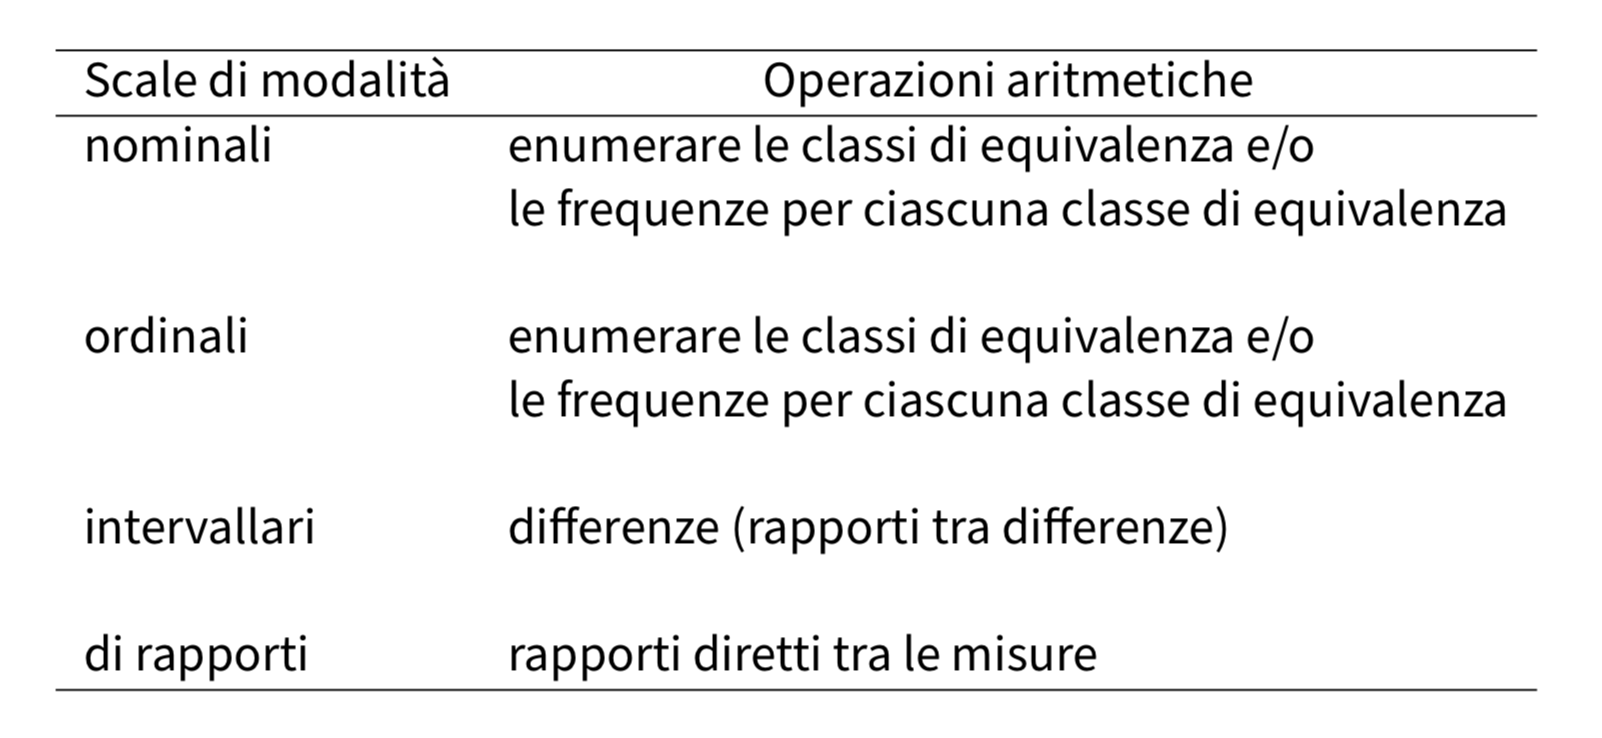
\includegraphics[width=0.7\linewidth,height=\textheight,keepaspectratio]{chapters/key_notions/../../figures/misurazione_2.png}

}

\caption{Scale di misurazione.}

\end{figure}%

\subsection{Scala nominale}\label{scala-nominale}

La scala nominale è il livello di misurazione più semplice e corrisponde
ad una tassonomia o classificazione delle categorie che utilizziamo per
descrivere i fenomeni psicologici. I simboli o numeri che costituiscono
questa scala rappresentano i nomi delle categorie e non hanno alcun
valore numerico intrinseco. Con la scala nominale possiamo solo
distinguere se una caratteristica psicologica è uguale o diversa da
un'altra.

I dati raccolti con la scala nominale sono suddivisi in categorie
qualitative e mutuamente esclusive, in cui ogni dato appartiene ad una
sola categoria. In questa scala, esiste solo la relazione di equivalenza
tra le misure delle unità di studio: gli elementi del campione
appartenenti a classi diverse sono differenti, mentre tutti quelli della
stessa classe sono tra loro equivalenti.

L'unica operazione algebrica consentita dalla scala nominale è quella di
contare le unità di studio che appartengono ad ogni categoria e il
numero totale di categorie. Di conseguenza, la descrizione dei dati
avviene tramite le frequenze assolute e le frequenze relative.

Dalla scala nominale è possibile costruire altre scale nominali
equivalenti alla prima, trasformando i valori della scala di partenza in
modo tale da cambiare i nomi delle categorie, ma lasciando inalterata la
suddivisione delle unità di studio nelle medesime classi di equivalenza.
In altre parole, cambiando i nomi delle categorie di una variabile
misurata su scala nominale, si ottiene una nuova variabile esattamente
equivalente alla prima.

\subsection{Scala ordinale}\label{scala-ordinale}

La scala ordinale mantiene la caratteristica della scala nominale di
classificare ogni unità di misura all'interno di una singola categoria,
ma introduce la relazione di ordinamento tra le categorie. In quanto
basata su una relazione di ordine, una scala ordinale descrive solo il
rango di ordine tra le categorie e non fornisce informazioni sulla
distanza tra di esse. Non ci dice, ad esempio, se la distanza tra le
categorie \(a\) e \(b\) è uguale, maggiore o minore della distanza tra
le categorie \(b\) e \(c\).

Un esempio classico di scala ordinale è quello della scala Mohs per la
determinazione della durezza dei minerali. Per stabilire la durezza dei
minerali si usa il criterio empirico della scalfittura. Vengono
stabiliti livelli di durezza crescente da 1 a 10 con riferimento a dieci
minerali: talco, gesso, calcite, fluorite, apatite, ortoclasio, quarzo,
topazio, corindone e diamante. Un minerale appartenente ad uno di questi
livelli se scalfisce quello di livello inferiore ed è scalfito da quello
di livello superiore.

\begin{figure}[H]

{\centering 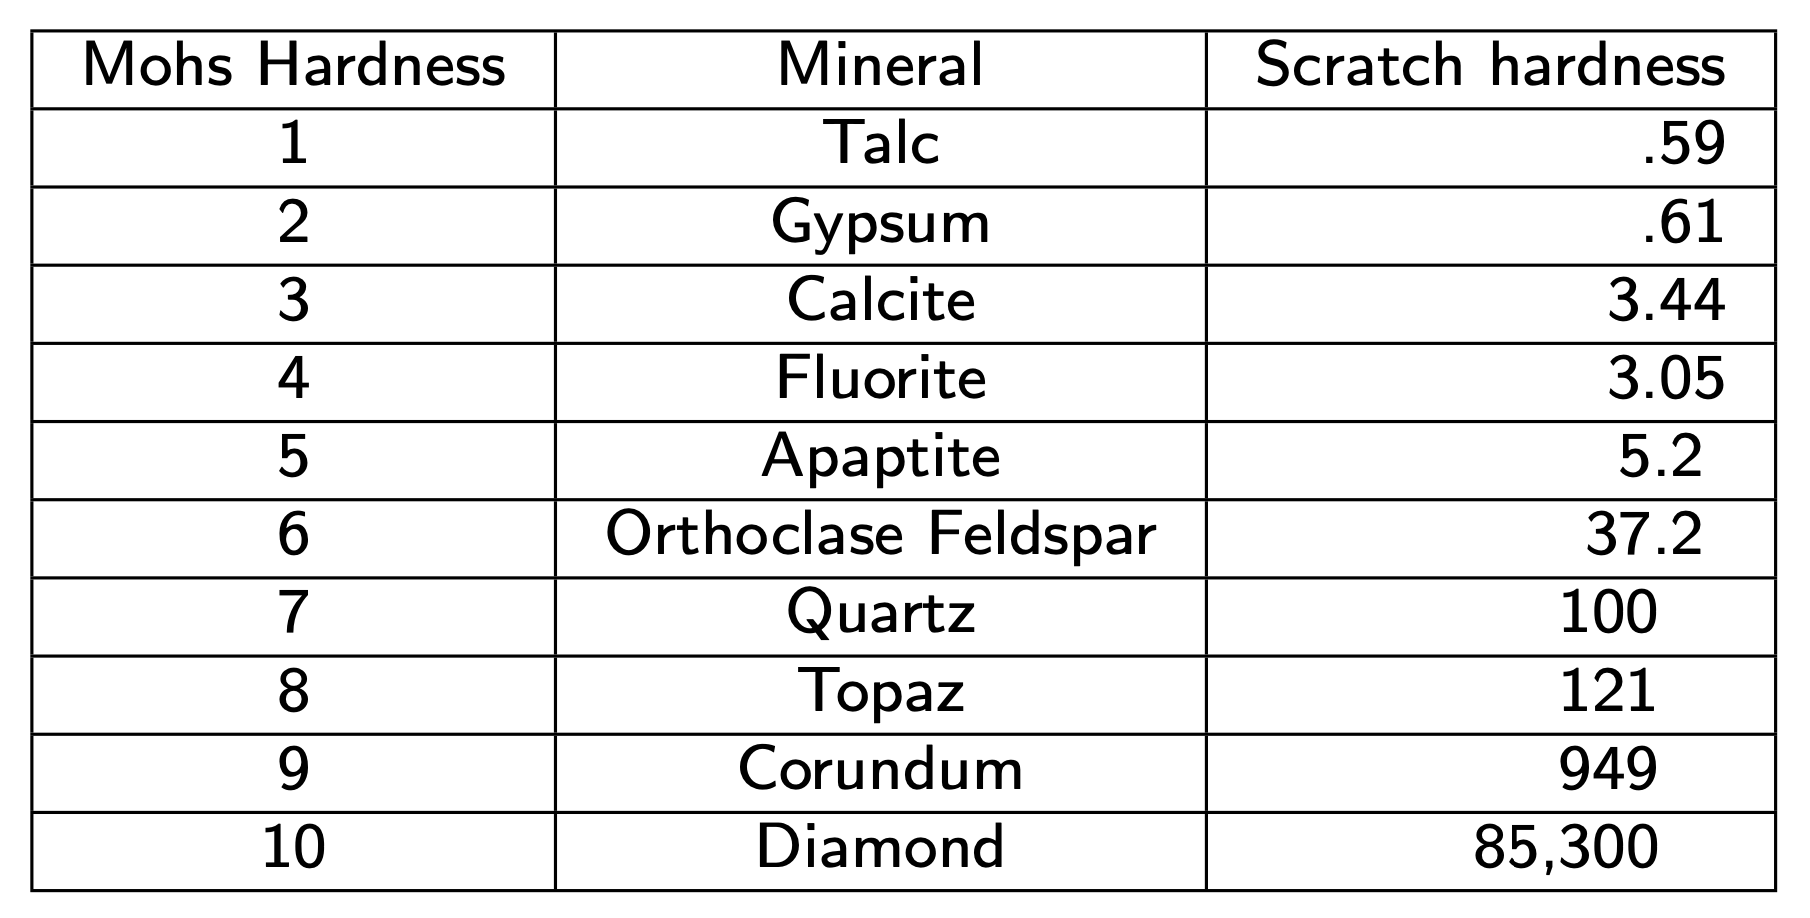
\includegraphics[width=0.62\linewidth,height=\textheight,keepaspectratio]{chapters/key_notions/../../figures/mohs.png}

}

\caption{La scala di durezza dei minerali di Mohs. Un oggetto è
considerato più duro di X se graffia X. Sono incluse anche misure di
durezza relativa utilizzando uno sclerometro, da cui emerge la non
linearità della scala di Mohs (Burchard, 2004).}

\end{figure}%

\subsection{Scala ad intervalli}\label{scala-ad-intervalli}

La scala ad intervalli di misurazione include le proprietà della scala
nominale e della scala ordinale e permette di misurare le distanze tra
le coppie di unità statistiche in termini di un intervallo costante,
chiamato ``unità di misura'', a cui viene attribuito il valore ``1''.
L'origine della scala, ovvero il punto zero, è scelta arbitrariamente e
non indica l'assenza della proprietà che si sta misurando. Ciò significa
che la scala ad intervalli consente anche valori negativi e lo zero non
viene attribuito all'unità statistica in cui la proprietà risulta
assente.

La scala ad intervalli equivalenti consente l'esecuzione di operazioni
algebriche basate sulla differenza tra i numeri associati ai diversi
punti della scala, operazioni algebriche non possibili con le scale di
misura nominale o ordinale. Tuttavia, il limite della scala ad
intervalli è che non consente di calcolare il rapporto tra coppie di
misure. È possibile affermare la differenza tra \(a\) e \(b\) come la
metà della differenza tra \(c\) e \(d\) o che le due differenze sono
uguali, ma non è possibile affermare che \(a\) abbia una proprietà
misurata in quantità doppia rispetto a \(b\). In altre parole, non è
possibile stabilire rapporti diretti tra le misure ottenute. Solo le
differenze tra le modalità permettono tutte le operazioni aritmetiche,
come la somma, l'elevazione a potenza o la divisione, che sono alla base
della statistica inferenziale.

Nelle scale ad intervalli equivalenti, l'unità di misura è arbitraria e
può essere cambiata attraverso una dilatazione, ovvero la
moltiplicazione di tutti i valori della scala per una costante positiva.
Inoltre, la traslazione, ovvero l'aggiunta di una costante a tutti i
valori della scala, è ammessa poiché non altera le differenze tra i
valori della scala. La scala rimane invariata rispetto a traslazioni e
dilatazioni e dunque le uniche trasformazioni ammissibili sono le
trasformazioni lineari:

\[
y' = a + by, \quad b > 0.
\]

Infatti, l'uguaglianza dei rapporti fra gli intervalli rimane invariata
a seguito di una trasformazione lineare.

Esempio di scala ad intervalli è la temperatura misurata in gradi
Celsius o Fahrenheit, ma non Kelvin. Come per la scala nominale, è
possibile stabilire se due modalità sono uguali o diverse:
\(30^\circ C \neq 20^\circ C\). Come per la scala ordinale è possibile
mettere due modalità in una relazione d'ordine:
\(30^\circ C > 20^\circ C\). In aggiunta ai casi precedenti, però, è
possibile definire una unità di misura per cui è possibile dire che tra
\(30^\circ C\) e \(20^\circ C\) c'è una differenza di
\(30^\circ - 20^\circ = 10^\circ C\). I valori di temperatura, oltre a
poter essere ordinati secondo l'intensità del fenomeno, godono della
proprietà che le differenze tra loro sono direttamente confrontabili e
quantificabili.

Il limite della scala ad intervalli è quello di non consentire il
calcolo del rapporto tra coppie di misure. Ad esempio, una temperatura
di \(80^\circ C\) non è il doppio di una di \(40^\circ C\). Se infatti
esprimiamo le stesse temperature nei termini della scala Fahrenheit,
allora i due valori non saranno in rapporto di 1 a 2 tra loro. Infatti,
\(20^\circ C = 68^\circ F\) e \(40^\circ C = 104^\circ F\). Questo
significa che la relazione ``il doppio di'' che avevamo individuato in
precedenza si applicava ai numeri della scala centigrada, ma non alla
proprietà misurata (cioè la temperatura). La decisione di che scala
usare (Centigrada vs.~Fahrenheit) è arbitraria. Ma questa arbitrarietà
non deve influenzare le inferenze che traiamo dai dati. Queste
inferenze, infatti, devono dirci qualcosa a proposito della realtà
empirica e non possono in nessun modo essere condizionate dalle nostre
scelte arbitrarie che ci portano a scegliere la scala Centigrada
piuttosto che quella Fahrenheit.

Consideriamo ora l'aspetto invariante di una trasformazione lineare,
ovvero l'uguaglianza dei rapporti fra intervalli. Prendiamo in esame, ad
esempio, tre temperature: \(20^\circ C = 68^\circ F\),
\(15^\circ C = 59^\circ F\), \(10^\circ C = 50 ^\circ F\).

È facile rendersi conto del fatto che i rapporti fra intervalli restano
costanti indipendentemente dall'unità di misura che è stata scelta:

\[
  \frac{20^\circ C - 10^\circ C}{20^\circ C - 15^\circ C} =
  \frac{68^\circ F - 50^\circ F}{68^\circ F-59^\circ F} = 2.
\]

\subsection{Scala di rapporti}\label{scala-di-rapporti}

Nella scala a rapporti equivalenti, lo zero non è arbitrario e
rappresenta l'elemento che ha intensità nulla rispetto alla proprietà
misurata. Per costruire questa scala, si associa il numero 0
all'elemento con intensità nulla e si sceglie un'unità di misura \(u\).
Ad ogni elemento si assegna un numero \(a\) definito come \(a = d / u\),
dove \(d\) rappresenta la distanza dall'origine. In questo modo, i
numeri assegnati riflettono le differenze e i rapporti tra le intensità
della proprietà misurata.

In questa scala, è possibile effettuare operazioni aritmetiche non solo
sulle differenze tra i valori della scala, ma anche sui valori stessi
della scala. L'unica scelta arbitraria è l'unità di misura, ma lo zero
deve sempre rappresentare l'intensità nulla della proprietà considerata.

Le trasformazioni ammissibili in questa scala sono chiamate
trasformazioni di similarità e sono del tipo \(y' = by\), dove
\(b > 0\). In questa scala, i rapporti tra i valori rimangono invariati
dopo le trasformazioni. In altre parole, se rapportiamo due valori
originali e due valori trasformati, il rapporto rimane lo stesso:
\(\frac{y_i}{y_j} = \frac{y'_i}{y'_j}\).

\section{Gerarchia dei livelli delle scale di
misurazione}\label{gerarchia-dei-livelli-delle-scale-di-misurazione}

Secondo Stevens (1946), esiste una gerarchia dei livelli delle scale di
misurazione, denominati ``livelli di scala''. Questi livelli sono
organizzati in modo gerarchico, in cui la scala nominale rappresenta il
livello più basso della misurazione, mentre la scala a rapporti
equivalenti rappresenta il livello più alto.

\begin{itemize}
\tightlist
\item
  \textbf{Scala nominale}: Classifica le categorie senza un ordine
  specifico.
\item
  \textbf{Scala ordinale}: Classifica le categorie in un ordine
  specifico, ma senza una misura precisa delle distanze.
\item
  \textbf{Scala a intervalli}: Misura le distanze tra le categorie con
  un intervallo costante, ma senza un punto zero assoluto.
\item
  \textbf{Scala di rapporti}: Misura le distanze con un intervallo
  costante e un punto zero assoluto.
\end{itemize}

\begin{figure}[H]

{\centering 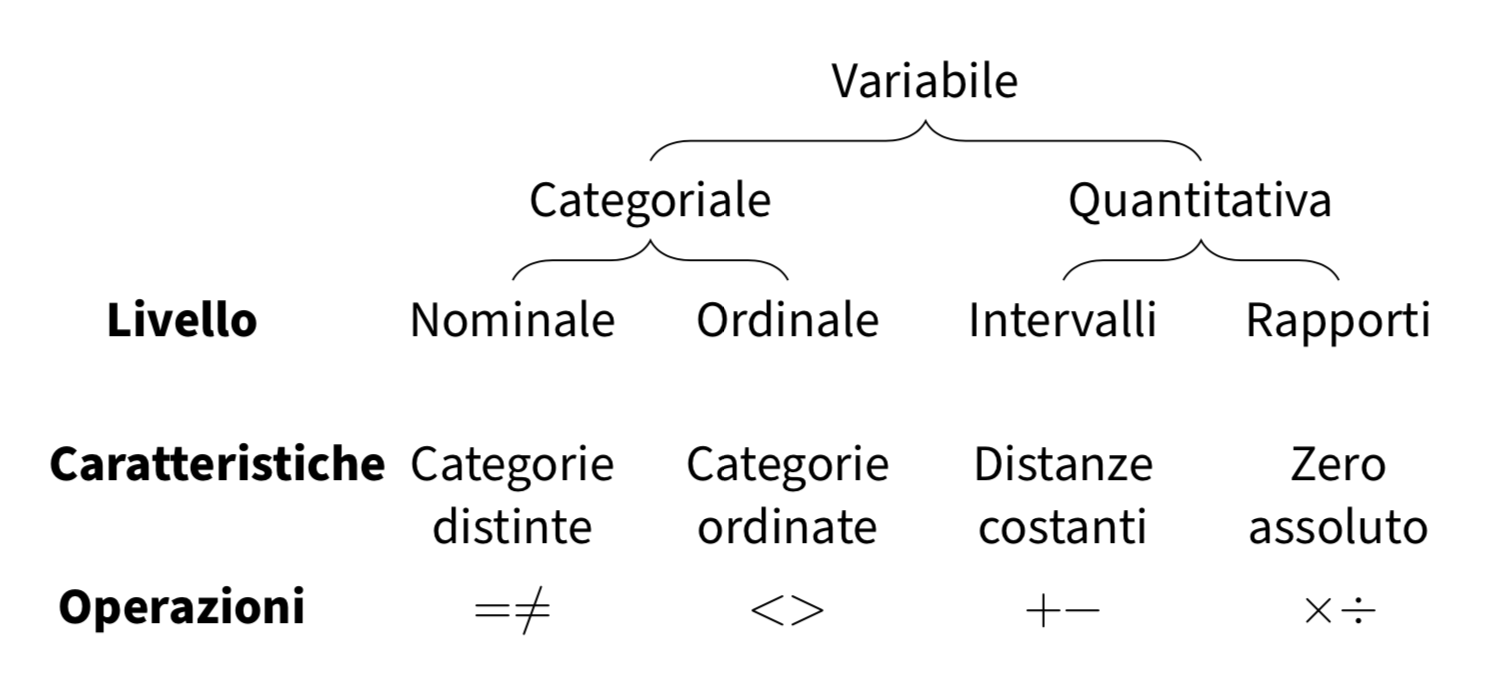
\includegraphics[width=0.65\linewidth,height=\textheight,keepaspectratio]{chapters/key_notions/../../figures/misurazione_1.png}

}

\caption{Relazioni tra i livelli di misurazione.}

\end{figure}%

Passando da un livello di misurazione ad uno più alto aumenta il numero
di operazioni aritmetiche che possono essere compiute sui valori della
scala.

\subsection{Variabili Discrete e
Continue}\label{variabili-discrete-e-continue}

Le variabili possono essere classificate come variabili a livello di
intervalli o di rapporti e possono essere sia discrete che continue.

\begin{itemize}
\tightlist
\item
  \textbf{Variabili discrete}: Assumono valori specifici ma non possono
  assumere valori intermedi.
\item
  \textbf{Variabili continue}: Possono assumere qualsiasi valore
  all'interno di un intervallo specificato.
\end{itemize}

\begin{figure}[H]

{\centering 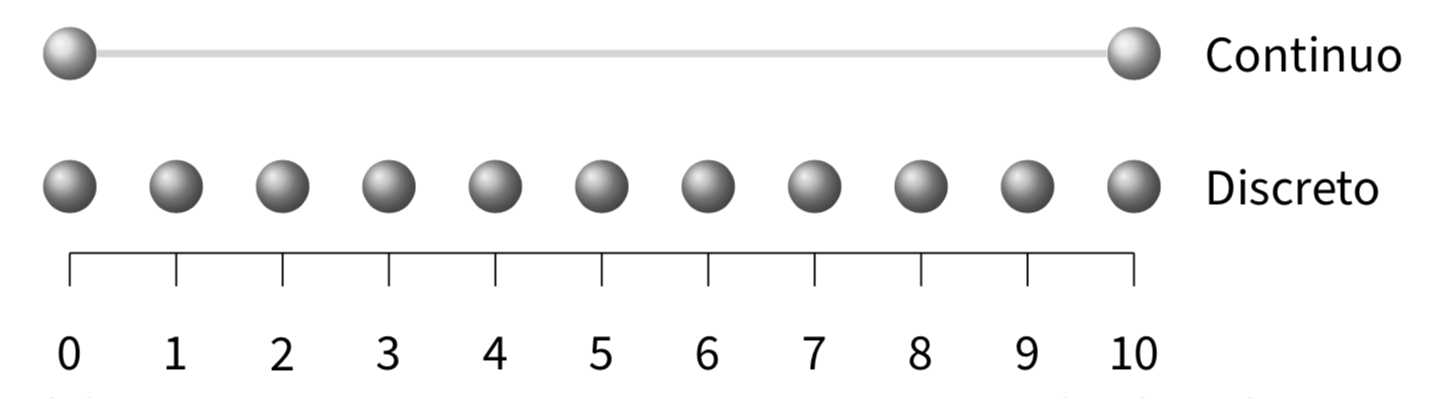
\includegraphics[width=0.65\linewidth,height=\textheight,keepaspectratio]{chapters/key_notions/../../figures/misurazione_3.png}

}

\caption{Variabili discrete e continue.}

\end{figure}%

\section{Riflessioni Conclusive}\label{riflessioni-conclusive-2}

La misurazione in psicologia non è un semplice atto di raccolta di dati,
ma un processo fondamentale per garantire che le osservazioni empiriche
siano interpretabili alla luce di modelli teorici solidi. Una buona
misurazione non si limita a ridurre l'errore, ma consente di attribuire
un significato coerente ai punteggi ottenuti, facilitando così il
progresso della conoscenza scientifica. Senza strumenti adeguati per la
misurazione, il rischio è quello di costruire teorie su basi incerte,
compromettendo la validità delle conclusioni tratte.

Due pilastri sostengono una ricerca psicologica rigorosa: la teoria e la
misurazione. La teoria fornisce il quadro concettuale entro cui si
interpretano i dati, definendo le ipotesi e orientando le analisi. La
\href{https://statmodeling.stat.columbia.edu/2015/04/28/whats-important-thing-statistics-thats-not-textbooks/}{misurazione},
invece, è il ponte tra i costrutti astratti e le osservazioni empiriche,
traducendo concetti complessi in variabili operative affidabili. Nessuna
delle due componenti può reggersi senza l'altra: una teoria senza
misurazione adeguata rischia di rimanere speculativa, mentre una
misurazione priva di un solido fondamento teorico può portare a dati
privi di significato.

Nella valutazione di un qualsiasi studio psicologico, un approccio
critico richiede quindi di esaminare sia la solidità del quadro teorico
sia la qualità degli strumenti di misurazione adottati. Il progresso
della ricerca dipende dalla capacità di integrare questi due elementi,
attraverso metodologie sempre più sofisticate che riducano l'incertezza
e migliorino la precisione delle inferenze. Le moderne tecniche di
analisi dei dati, i modelli psicometrici avanzati e le tecnologie
digitali stanno ampliando le possibilità di misurazione, offrendo
strumenti più sensibili e adattabili alla complessità dei fenomeni
psicologici. Tuttavia, la sfida principale rimane la stessa: garantire
che la misurazione sia non solo accurata, ma anche teoricamente fondata,
affinché le conoscenze acquisite possano davvero contribuire alla
comprensione della mente e del comportamento umano.

\section*{Esercizio}\label{esercizio}
\addcontentsline{toc}{section}{Esercizio}

\markright{Esercizio}

Un esempio di come condurre una lettura critica è rappresentato
dall'analisi di un articolo scientifico pubblicato su \emph{Nature} sul
tema del \textbf{mind-body healing}
(\citeproc{ref-aungle2023physical}{Aungle \& Langer, 2023}). Lo
\href{https://www.nature.com/articles/s41598-023-50009-3}{studio} in
questione presenta risultati empirici che suggeriscono un legame tra
pratiche di guarigione mente-corpo e miglioramenti nella salute fisica.
Tuttavia, la validità di queste conclusioni è stata fortemente
contestata da Andrew Gelman, un noto statistico e ricercatore, in un
post sul suo blog
\href{https://statmodeling.stat.columbia.edu/2025/01/27/does-anyone-actually-expect-meaningful-insight-to-come-from-a-study-like-this/}{Statistical
Modeling}.

Gelman sottolinea un aspetto cruciale della ricerca scientifica:
l'importanza di una \textbf{teoria sostanziale solida e convincente}.
Secondo il suo punto di vista, lo studio analizzato presenta una carenza
significativa in questo ambito. In assenza di una teoria ben fondata che
spieghi in modo plausibile i meccanismi causali attraverso cui le
pratiche mente-corpo potrebbero influenzare la salute fisica, i
risultati empirici ottenuti rimangono privi di significato. Senza una
cornice teorica coerente, lo studio rischia di essere classificato come
ciò che Gelman definisce ``junk science'' -- scienza di scarso valore,
incapace di offrire vere e proprie intuizioni.

Una teoria sostanziale non deve solo essere plausibile, ma deve anche
integrarsi in modo coerente con altre teorie scientifiche consolidate.
Quando una ricerca non riesce a inserirsi in una rete più ampia di
conoscenze, i suoi risultati diventano inevitabilmente discutibili. È
proprio questo il caso dello studio esaminato da Gelman: l'assenza di
una teoria chiara e ben articolata rende i risultati empirici poco
credibili e difficilmente generalizzabili.

Oltre alla debolezza teorica, lo studio presenta anche problemi
significativi legati alla \textbf{misurazione}. Le variabili utilizzate
per quantificare sia gli interventi mente-corpo che gli esiti sanitari
sono soggette a diverse criticità. Ad esempio, la misurazione
dell'efficacia delle pratiche mente-corpo potrebbe essere influenzata da
fattori confondenti, come le aspettative dei partecipanti o l'effetto
placebo. Allo stesso modo, la valutazione degli esiti sanitari può
risultare problematica se non vengono impiegate scale di misurazione
affidabili e valide.

Per un approfondimento su questi temi, si rimanda alle riflessioni
conclusive nella sezione \textbf{?@sec-prob-sampling-distr}, dove
vengono discusse criticamente le questioni legate alla misurazione, con
particolare attenzione alla distinzione tra
\href{https://en.wikipedia.org/wiki/Accuracy_and_precision}{precisione e
bias}. In generale, uno degli aspetti più critici della misurazione
riguarda la validità
\href{https://en.wikipedia.org/wiki/Internal_validity}{interna} ed
\href{https://en.wikipedia.org/wiki/External_validity}{esterna} negli
studi psicologici. La qualità delle misure adottate influisce
direttamente sulla solidità delle conclusioni scientifiche: una
misurazione imprecisa o distorta può compromettere la validità dei
risultati e limitarne la generalizzabilità.

L'esempio dello studio sul mind-body healing illustra in modo efficace
come una lettura critica debba necessariamente passare attraverso due
dimensioni fondamentali: la \textbf{teoria} e la \textbf{misurazione}.
Una teoria debole compromette la capacità di attribuire significato ai
dati raccolti, riducendo lo studio a una mera raccolta di numeri privi
di valore scientifico. Allo stesso tempo, problemi di misurazione
possono distorcere i risultati, portando a conclusioni errate o
fuorvianti. Solo attraverso una valutazione attenta di entrambi questi
aspetti è possibile distinguere tra ricerche scientificamente valide e
``junk science''.

In definitiva, una lettura critica di un articolo psicologico richiede
non solo competenze tecniche, ma anche una profonda consapevolezza dei
limiti e delle sfide insite nella misurazione psicologica e nel rapporto
tra misurazione e teorie scientifiche. Questo approccio consente di
valutare in modo equilibrato la qualità e l'affidabilità delle
conclusioni proposte.

\section*{Bibliografia}\label{bibliografia-3}
\addcontentsline{toc}{section}{Bibliografia}

\markright{Bibliografia}

\chapter{La riforma metodologica in psicologia: dalla crisi alla
rivoluzione bayesiana}\label{sec-data-science}

\begin{tcolorbox}[enhanced jigsaw, toprule=.15mm, breakable, bottomrule=.15mm, colback=white, colbacktitle=quarto-callout-important-color!10!white, left=2mm, toptitle=1mm, colframe=quarto-callout-important-color-frame, coltitle=black, opacitybacktitle=0.6, bottomtitle=1mm, titlerule=0mm, leftrule=.75mm, opacityback=0, rightrule=.15mm, title=\textcolor{quarto-callout-important-color}{\faExclamation}\hspace{0.5em}{In questo capitolo imparerai a}, arc=.35mm]

\begin{itemize}
\tightlist
\item
  comprendere il contesto storico e concettuale della trasformazione
  metodologica in psicologia;
\item
  identificare le principali criticità metodologiche che hanno
  contribuito alla crisi di replicabilità;
\item
  descrivere l'approccio bayesiano come paradigma statistico alternativo
  al frequentismo.
\end{itemize}

\end{tcolorbox}

\begin{tcolorbox}[enhanced jigsaw, toprule=.15mm, breakable, bottomrule=.15mm, colback=white, colbacktitle=quarto-callout-tip-color!10!white, left=2mm, toptitle=1mm, colframe=quarto-callout-tip-color-frame, coltitle=black, opacitybacktitle=0.6, bottomtitle=1mm, titlerule=0mm, leftrule=.75mm, opacityback=0, rightrule=.15mm, title=\textcolor{quarto-callout-tip-color}{\faLightbulb}\hspace{0.5em}{Prerequisiti}, arc=.35mm]

\begin{itemize}
\tightlist
\item
  Leggere \emph{Statistical Rethinking}
  (\citeproc{ref-McElreath_rethinking}{McElreath, 2020}). Focalizzati
  sui primi capitoli dove si discute della dicotomia tra ``small world''
  e ``big world''.
\item
  Leggere
  \href{https://statmodeling.stat.columbia.edu/2016/09/21/what-has-happened-down-here-is-the-winds-have-changed/}{What
  has happened down here is the winds have changed (Gelman 2016)}. Un
  post sul blog di Andrew Gelman che fornisce una panoramica sulla crisi
  di replicazione e su come le scienze sociali sono cambiate di
  conseguenza.
\item
  Leggere
  \href{https://psycnet.apa.org/fulltext/2025-04988-001.html}{Productive
  Explanation: A Framework for Evaluating Explanations in Psychological
  Science}. L'adozione di teorie formali è essenziale per affrontare la
  crisi di riproducibilità dei risultati nella ricerca psicologica.
\item
  Per chi fosse interessato a un romanzo su questi temi,
  sorprendentemente avvincente, consiglio \emph{Quando abbiamo smesso di
  capire il mondo} di Benjamín Labatut
  (\citeproc{ref-labatut2021abbiamo}{Labatut, 2021}).
\end{itemize}

\end{tcolorbox}

\section*{Introduzione}\label{introduzione-3}
\addcontentsline{toc}{section}{Introduzione}

\markright{Introduzione}

Negli ultimi vent'anni, le scienze sociali e la psicologia hanno vissuto
una profonda trasformazione metodologica ed epistemologica. Questo
cambiamento, spesso definito come ``Credibility Revolution''
(\citeproc{ref-angrist2010credibility}{Angrist \& Pischke, 2010}),
``Causal Revolution'' (\citeproc{ref-pearl2018book}{Pearl \& Mackenzie,
2018}) e ``Replication Crisis''
(\citeproc{ref-open2015estimating}{Collaboration, 2015};
\citeproc{ref-nosek2022replicability}{Nosek et al., 2022}), ha portato a
un ripensamento delle pratiche di ricerca, specialmente in psicologia
(\citeproc{ref-korbmacher2023replication}{Korbmacher et al., 2023}).
Questa transizione verso quella che Munger
(\citeproc{ref-munger2023temporal}{2023}) chiama ``Science versione 2''
è stata motivata dalla consapevolezza di lacune metodologiche passate e
ha spinto verso l'adozione di approcci più rigorosi e replicabili.

Le origini di questa riforma risiedono nel riconoscimento di problemi
metodologici diffusi, come la proliferazione di falsi positivi
(\citeproc{ref-simmons2011false}{Simmons et al., 2011}), l'abuso dei
``gradi di libertà dei ricercatori''
(\citeproc{ref-gelman2013garden}{Gelman \& Loken, 2013}), e
l'inadeguatezza delle pratiche statistiche tradizionali
(\citeproc{ref-gelman2014statistical}{Gelman \& Loken, 2014}). Fenomeni
come il p-hacking, l'uso di campioni di piccole dimensioni
(\citeproc{ref-button2013power}{Button et al., 2013}), e la mancanza di
trasparenza nei metodi di ricerca hanno contribuito a minare la
credibilità delle scoperte psicologiche
(\citeproc{ref-ioannidis2005most}{Ioannidis, 2005};
\citeproc{ref-meehl1967theory}{Meehl, 1967}), portando alla cosiddetta
``Replication Crisis'' (\citeproc{ref-baker20161}{Baker, 2016};
\citeproc{ref-bishop2019psychology}{Bishop, 2019}) --- si veda il
\textbf{?@sec-crisis-replication}.

\section{L'Approccio Bayesiano}\label{lapproccio-bayesiano}

In risposta a queste sfide, l'approccio bayesiano è emerso come un
paradigma statistico chiave nella ``Credibility Revolution''. A
differenza dell'inferenza frequentista, che si basa sul Test
dell'Ipotesi Nulla, la statistica bayesiana offre un framework più
flessibile e intuitivo per l'analisi dei dati e l'inferenza causale. Il
principio fondamentale dell'approccio bayesiano è l'aggiornamento delle
distribuzioni di probabilità a priori (priors) alla luce di nuove
evidenze, un processo che si allinea con l'obiettivo di una scienza
cumulativa e auto-correttiva.

L'adozione di metodi bayesiani in psicologia presenta numerosi vantaggi:

\begin{enumerate}
\def\labelenumi{\arabic{enumi}.}
\tightlist
\item
  \textbf{Quantificazione dell'incertezza}: L'inferenza bayesiana
  fornisce distribuzioni di probabilità posteriori complete per i
  parametri di interesse, offrendo una rappresentazione più ricca e
  sfumata dell'incertezza rispetto agli intervalli di confidenza
  frequentisti.
\item
  \textbf{Incorporazione di conoscenze pregresse}: Le priors bayesiane
  permettono di integrare formalmente conoscenze precedenti nel processo
  inferenziale, promuovendo un approccio cumulativo alla ricerca.
\item
  \textbf{Robustezza alle pratiche di ricerca discutibili}: I metodi
  bayesiani sono meno suscettibili a pratiche come il p-hacking, poiché
  l'inferenza si basa sull'intera distribuzione posteriore piuttosto che
  su soglie arbitrarie di significatività.
\end{enumerate}

\section{L'Approccio Bayesiano nella Ricerca
Psicologica}\label{lapproccio-bayesiano-nella-ricerca-psicologica}

L'uso delle statistiche bayesiane nella ricerca psicologica offre
vantaggi significativi rispetto ai metodi statistici tradizionali, come
il test di significatività dell'ipotesi nulla. Uno dei punti di forza
principali è la sua indipendenza dalla teoria dei grandi campioni,
rendendolo particolarmente adatto per studi che spesso si basano su
campioni di dimensioni ridotte (\citeproc{ref-larson2023bayesian}{Larson
et al., 2023}).

La ricerca psicologica è spesso caratterizzata da campioni limitati,
dovuti a fattori come la bassa prevalenza di determinate condizioni,
difficoltà nel reclutamento dei partecipanti e complessità nelle
procedure di valutazione. Questi campioni di piccole dimensioni sono
intrinsecamente soggetti a una maggiore eterogeneità, che si manifesta
nella variabilità del fenotipo comportamentale delle condizioni
psicologiche esaminate e nella discrepanza tra le stime degli effetti in
diversi studi. Tale eterogeneità può portare a stime degli effetti
distorte e scarsamente riproducibili.

L'approccio bayesiano offre una soluzione efficace a queste
problematiche. In primo luogo, consente di valutare l'adeguatezza della
dimensione del campione attraverso un'analisi della sensibilità dei
risultati rispetto alla specificazione delle distribuzioni a priori. In
secondo luogo, permette di ottenere risultati precisi anche con campioni
ridotti, a condizione che le conoscenze a priori siano accurate e ben
definite.

Un ulteriore vantaggio è la capacità dell'approccio bayesiano di
ottimizzare l'uso dei campioni di partecipanti, favorendo un'inclusione
equa delle popolazioni diversificate. Questo è particolarmente rilevante
per gruppi spesso sottorappresentati, come le minoranze etniche. Le
statistiche bayesiane aiutano a superare questa sfida evitando di
esercitare una pressione eccessiva su questi gruppi per aumentarne la
partecipazione, permettendo così una ricerca più equa e rappresentativa.

\section{Modellazione Formale e Data
Science}\label{modellazione-formale-e-data-science}

La ``Credibility Revolution'' ha favorito l'integrazione della Data
Science nelle pratiche di ricerca psicologica. L'adozione di pipeline di
analisi dei dati riproducibili, l'uso di controllo di versione e la
condivisione di dati e codice sono diventati standard de facto nella
comunità scientifica. Questi strumenti non solo migliorano la
trasparenza e la replicabilità della ricerca, ma facilitano anche la
collaborazione e l'accumulo di conoscenze nel campo.

Parallelamente, si è osservato un rinnovato interesse per la
modellazione formale in psicologia, che consente non solo la verifica ma
anche lo sviluppo di modelli dei meccanismi sottostanti ai fenomeni
psicologici (\citeproc{ref-oberauer2019addressing}{Oberauer \&
Lewandowsky, 2019}; \citeproc{ref-van2024productive}{Van Dongen et al.,
2024}). Questo approccio supera la mera descrizione delle associazioni
tra variabili, tipica della pratica dominante dell'ANOVA nel contesto
pre-riforma.

La modellazione bayesiana si presta particolarmente bene a questo
approccio, offrendo un framework unificato per la specificazione di
modelli formali, l'incorporazione di incertezza parametrica e la
valutazione dell'evidenza empirica. Attraverso tecniche come il
confronto tra modelli bayesiano e l'analisi di sensibilità, i
ricercatori possono valutare rigorosamente la plausibilità relativa di
diverse teorie psicologiche.

\section{Riflessioni Epistemologiche}\label{riflessioni-epistemologiche}

L'adozione di metodi bayesiani e della Data Science in psicologia deve
essere accompagnata da una profonda riflessione epistemologica. Come
sottolineato da George Box:

\begin{quote}
Tutti i modelli sono sbagliati, ma alcuni sono utili.
\end{quote}

Questa massima risuona particolarmente nel contesto della ricerca
psicologica, dove i fenomeni di interesse sono spesso complessi e
multifattoriali.

L'approccio bayesiano, con la sua enfasi sull'aggiornamento iterativo
delle credenze alla luce di nuove evidenze, si allinea naturalmente con
una visione della scienza come processo di apprendimento continuo
piuttosto che come ricerca di verità assolute. Questa prospettiva
riconosce i limiti intrinseci dei nostri modelli e delle nostre teorie,
pur valorizzandone l'utilità euristica e predittiva.

In particolare, McElreath (\citeproc{ref-McElreath_rethinking}{2020})
sottolinea l'importanza di riconoscere la dualità tra il ``mondo del
modello'' e il mondo reale più ampio che cerchiamo di comprendere.
Questa consapevolezza è cruciale per evitare la reificazione dei nostri
modelli statistici e per mantenere una prospettiva critica sulle nostre
inferenze.

\section{Riflessioni Conclusive}\label{riflessioni-conclusive-3}

L'integrazione dell'approccio bayesiano e della Data Science nella
ricerca psicologica rappresenta una risposta promettente alle sfide
poste dalla ``Replication Crisis''. Offrendo un framework coerente per
la modellazione formale, l'inferenza statistica e l'incorporazione di
conoscenze pregresse, questi approcci promettono di elevare il rigore e
la credibilità della ricerca psicologica. Tuttavia, è fondamentale che
l'adozione di questi metodi sia accompagnata da una adeguata
consapevolezza metodologica ed epistemologica.

\section*{Bibliografia}\label{bibliografia-4}
\addcontentsline{toc}{section}{Bibliografia}

\markright{Bibliografia}

\phantomsection\label{refs}
\begin{CSLReferences}{1}{0}
\bibitem[\citeproctext]{ref-angrist2010credibility}
Angrist, J. D., \& Pischke, J.-S. (2010). The credibility revolution in
empirical economics: How better research design is taking the con out of
econometrics. \emph{Journal of economic perspectives}, \emph{24}(2),
3--30.

\bibitem[\citeproctext]{ref-aungle2023physical}
Aungle, P., \& Langer, E. (2023). Physical healing as a function of
perceived time. \emph{Scientific Reports}, \emph{13}(1), 22432.

\bibitem[\citeproctext]{ref-baker20161}
Baker, M. (2016). 1,500 scientists lift the lid on reproducibility.
\emph{Nature}, \emph{533}(7604).

\bibitem[\citeproctext]{ref-bishop2019psychology}
Bishop, D. (2019). \emph{The psychology of experimental psychologists:
Overcoming cognitive constraints to improve research}.

\bibitem[\citeproctext]{ref-button2013power}
Button, K. S., Ioannidis, J. P., Mokrysz, C., Nosek, B. A., Flint, J.,
Robinson, E. S., \& Munafò, M. R. (2013). Power failure: why small
sample size undermines the reliability of neuroscience. \emph{Nature
Reviews Neuroscience}, \emph{14}(5), 365--376.

\bibitem[\citeproctext]{ref-open2015estimating}
Collaboration, O. S. (2015). Estimating the reproducibility of
psychological science. \emph{Science}, \emph{349}(6251), aac4716.

\bibitem[\citeproctext]{ref-funder2014improving}
Funder, D. C., Levine, J. M., Mackie, D. M., Morf, C. C., Sansone, C.,
Vazire, S., \& West, S. G. (2014). Improving the dependability of
research in personality and social psychology: Recommendations for
research and educational practice. \emph{Personality and Social
Psychology Review}, \emph{18}(1), 3--12.

\bibitem[\citeproctext]{ref-gelman1995bayesian}
Gelman, A., Carlin, J. B., Stern, H. S., \& Rubin, D. B. (1995).
\emph{Bayesian data analysis}. Chapman; Hall/CRC.

\bibitem[\citeproctext]{ref-gelman2021regression}
Gelman, A., Hill, J., \& Vehtari, A. (2021). \emph{Regression and other
stories}. Cambridge University Press.

\bibitem[\citeproctext]{ref-gelman2013garden}
Gelman, A., \& Loken, E. (2013). The garden of forking paths: Why
multiple comparisons can be a problem, even when there is no {«fishing
expedition»} or {«p-hacking»} and the research hypothesis was posited
ahead of time. \emph{Department of Statistics, Columbia University},
\emph{348}(1-17), 3.

\bibitem[\citeproctext]{ref-gelman2014statistical}
Gelman, A., \& Loken, E. (2014). The statistical crisis in science.
\emph{American scientist}, \emph{102}(6), 460--465.

\bibitem[\citeproctext]{ref-huntington2021effect}
Huntington-Klein, N. (2021). \emph{The effect: An introduction to
research design and causality}. Chapman; Hall/CRC.

\bibitem[\citeproctext]{ref-ioannidis2005most}
Ioannidis, J. P. (2005). Why most published research findings are false.
\emph{PLoS medicine}, \emph{2}(8), e124.

\bibitem[\citeproctext]{ref-ioannidis2019have}
Ioannidis, J. P. (2019). What have we (not) learnt from millions of
scientific papers with P values? \emph{The American Statistician},
\emph{73}(sup1), 20--25.

\bibitem[\citeproctext]{ref-korbmacher2023replication}
Korbmacher, M., Azevedo, F., Pennington, C. R., Hartmann, H., Pownall,
M., Schmidt, K., Elsherif, M., Breznau, N., Robertson, O., Kalandadze,
T., et al. (2023). The replication crisis has led to positive
structural, procedural, and community changes. \emph{Communications
Psychology}, \emph{1}(1), 3.

\bibitem[\citeproctext]{ref-labatut2021abbiamo}
Labatut, B. (2021). \emph{Quando abbiamo smesso di capire il mondo}.
Adelphi Edizioni spa.

\bibitem[\citeproctext]{ref-larson2023bayesian}
Larson, C., Kaplan, D., Girolamo, T., Kover, S. T., \& Eigsti, I.-M.
(2023). A Bayesian statistics tutorial for clinical research: Prior
distributions and meaningful results for small clinical samples.
\emph{Journal of Clinical Psychology}, \emph{79}(11), 2602--2624.

\bibitem[\citeproctext]{ref-lilienfeld2020psychological}
Lilienfeld, S. O., \& Strother, A. N. (2020). Psychological measurement
and the replication crisis: Four sacred cows. \emph{Canadian
Psychology/Psychologie Canadienne}, \emph{61}(4), 281--288.

\bibitem[\citeproctext]{ref-maul2016philosophical}
Maul, A., Irribarra, D. T., \& Wilson, M. (2016). On the philosophical
foundations of psychological measurement. \emph{Measurement}, \emph{79},
311--320.

\bibitem[\citeproctext]{ref-McElreath_rethinking}
McElreath, R. (2020). \emph{Statistical rethinking: {A} {Bayesian}
course with examples in {R} and {Stan}} (2nd Edition). CRC Press.

\bibitem[\citeproctext]{ref-meehl1967theory}
Meehl, P. E. (1967). Theory-testing in psychology and physics: A
methodological paradox. \emph{Philosophy of science}, \emph{34}(2),
103--115.

\bibitem[\citeproctext]{ref-munger2023temporal}
Munger, K. (2023). Temporal validity as meta-science. \emph{Research \&
Politics}, \emph{10}(3), 20531680231187271.

\bibitem[\citeproctext]{ref-murray2024measuring}
Murray, E. J., \& Carr, K. C. (2024). Measuring Racial Sentiment Using
Social Media Is Harder Than It Seems. \emph{Epidemiology}, \emph{35}(1),
60--63.

\bibitem[\citeproctext]{ref-nobles2000shades}
Nobles, M. (2000). \emph{Shades of citizenship: Race and the census in
modern politics}. Stanford University Press.

\bibitem[\citeproctext]{ref-nosek2022replicability}
Nosek, B. A., Hardwicke, T. E., Moshontz, H., Allard, A., Corker, K. S.,
Dreber, A., Fidler, F., Hilgard, J., Kline Struhl, M., Nuijten, M. B.,
et al. (2022). Replicability, robustness, and reproducibility in
psychological science. \emph{Annual Review of Psychology}, \emph{73}(1),
719--748.

\bibitem[\citeproctext]{ref-oberauer2019addressing}
Oberauer, K., \& Lewandowsky, S. (2019). Addressing the theory crisis in
psychology. \emph{Psychonomic Bulletin \& Review}, \emph{26},
1596--1618.

\bibitem[\citeproctext]{ref-pearl2018book}
Pearl, J., \& Mackenzie, D. (2018). \emph{The book of why: the new
science of cause and effect}. Basic books.

\bibitem[\citeproctext]{ref-shrout2018psychology}
Shrout, P. E., \& Rodgers, J. L. (2018). Psychology, science, and
knowledge construction: Broadening perspectives from the replication
crisis. \emph{Annual Review of Psychology}, \emph{69}(1), 487--510.

\bibitem[\citeproctext]{ref-simmons2011false}
Simmons, J. P., Nelson, L. D., \& Simonsohn, U. (2011). False-positive
psychology: Undisclosed flexibility in data collection and analysis
allows presenting anything as significant. \emph{Psychological science},
\emph{22}(11), 1359--1366.

\bibitem[\citeproctext]{ref-tackett2019psychology}
Tackett, J. L., Brandes, C. M., King, K. M., \& Markon, K. E. (2019).
Psychology's replication crisis and clinical psychological science.
\emph{Annual Review of Clinical Psychology}, \emph{15}(1), 579--604.

\bibitem[\citeproctext]{ref-van2024productive}
Van Dongen, N., Bork, R. van, Finnemann, A., Haslbeck, J., Maas, H. L.
van der, Robinaugh, D. J., Ron, J. de, Sprenger, J., \& Borsboom, D.
(2024). Productive explanation: A framework for evaluating explanations
in psychological science. \emph{Psychological Review}.

\bibitem[\citeproctext]{ref-wagenmakers2018bayesian}
Wagenmakers, E.-J., Marsman, M., Jamil, T., Ly, A., Verhagen, J., Love,
J., Selker, R., Gronau, Q. F., Šmı́ra, M., Epskamp, S., et al. (2018).
Bayesian inference for psychology. Part I: Theoretical advantages and
practical ramifications. \emph{Psychonomic Bulletin \& Review},
\emph{25}, 35--57.

\bibitem[\citeproctext]{ref-yarkoni2022generalizability}
Yarkoni, T. (2022). The generalizability crisis. \emph{Behavioral and
Brain Sciences}, \emph{45}, e1.

\bibitem[\citeproctext]{ref-youyou2023discipline}
Youyou, W., Yang, Y., \& Uzzi, B. (2023). A discipline-wide
investigation of the replicability of Psychology papers over the past
two decades. \emph{Proceedings of the National Academy of Sciences},
\emph{120}(6), e2208863120.

\end{CSLReferences}




\end{document}
